%\documentclass{llncs}
\documentclass[runningheads,a4paper]{llncs}

%\documentclass{article}
%\usepackage[french]{babel}
\usepackage[latin1]{inputenc}
\usepackage{graphicx,graphics,epsfig,xypic}
%\usepackage{Parallel}
%\usepackage{psfrag}
\usepackage[usenames]{color}
\usepackage{latexsym}
\usepackage{amsfonts,amssymb,amsmath}
\usepackage{verbatim,theorem}
\usepackage{longtable}
\usepackage{tabularx}
%\usepackage{mathenv}
\usepackage{floatflt}
%\usepackage{gastex}

%%%%% GILADAS %%%%%%%%%%%%
\newcommand{\alarm}[1]{\marginpar{#1}}


%%%%%%%%%%%%%%%%%%%%%%%%%%%
\newcommand{\infr}[2]{\textstyle \frac{\stackrel{\textstyle #1}{}}{\stackrel{}{\textstyle #2}}}

\newcommand{\redsIMP}{\leadsto}
\newcommand{\redsADV}[1]{\overset{\mbox{\tiny%
$#1$}}{\Rightarrow}}
\newcommand{\redsADVX}[2]{\underset{\mbox{\tiny $#2$}}{\overset{\mbox{\tiny%
$#1$}}{\Rightarrow}}}
\newcommand{\redsADVb}[1]{\redsADVX{#1}{\bot}}
\newcommand{\redsADVt}[1]{\redsADVX{#1}{\top}}
\newcommand{\redsAOP}[1]{\overset{\mbox{\tiny $#1$}}\Uparrow}



%%%% AOP Syntax %%%%%%%
\newcommand{\langfont}{\mathtt}

\newcommand{\Skip}{\langfont{skip}}
\newcommand{\Abort}{\langfont{abort}}
\newcommand{\Assign}[2]{#1\langfont{:=}#2}
\newcommand{\Seq}{\langfont{;}}
\newcommand{\If}[3]{\langfont{if}~#1~\langfont{then}~#2~\langfont{else}~#3}
\newcommand{\While}[2]{\langfont{while}~#1~\langfont{do}~#2}
\newcommand{\Call}[3]{#1\langfont{:=}#2(#3)}
\newcommand{\Return}[1]{\langfont{return}~#1}
\newcommand{\Sreturn}{\langfont{return}}

\newcommand{\Proceed}[2]{#1\langfont{:=proceed}(#2)}
\newcommand{\Sproceed}{\langfont{proceed}}

\newcommand{\VarSet}{\mathcal{V}}
\newcommand{\FSet}{\mathcal{F}}
\newcommand{\ASet}{\mathcal{A}}
\newcommand{\bop}{\mathsf{bop}}
\newcommand{\rop}{\mathsf{rop}}
\newcommand{\iop}{\mathsf{op}}
\newcommand{\cflow}{\mathsf{cflow}}

%%%% STATE and frames, etc.. %%%%%%%%%%
% command, locals, globals
\newcommand{\atuple}[3]{\langle #1,\istate{#2}{#3} \rangle}
\newcommand{\wtuple}[3]{\langle #1, \istate{#2}{#3} \rangle}

% locals, globals
\newcommand{\istate}[2]{\llparenthesis #1,#2 \rrparenthesis}

% value,  globals
\newcommand{\fstate}[2]{\Langle #1, #2 \Rangle}


%%% 
\newcommand{\emptylist}{[\,]}
\newcommand{\cons}{\triangleright}
\newcommand{\semantics}[1]{\llbracket #1 \rrbracket}


%%%% Function declaration %%%%%%%%%%%

%% \newcommand{\Pre}{\varphi}
%% \newcommand{\Post}{\psi}
\newcommand{\Assert}{\phi}
%% \newcommand{\Pmap}{\vec{\Lambda} }
%% \newcommand{\fundecl}[6]{\{{#1};~ {#2};~{#3};~{#4};~{#5};~{#6}\}}
%% \newcommand{\Fundecl}
%%  {\fundecl{\vec{r}}{\Pre}{G}{\Post}{\PR}{\Pmap}}

%% Assertions
%% \newcommand{\Acmp}{\triangleleft}
\newcommand{\True}{\mathsf{true}}
\newcommand{\False}{\mathsf{false}}
\newcommand{\Aand}{\wedge}
\newcommand{\Aor}{\vee}
\newcommand{\Aneg}{\neg}
\newcommand{\Aimp}{\!\Rightarrow\!}
%% \newcommand{\subst}[2]{\{#1\!\leftarrow\!#2\}}
\newcommand{\res}{{\sf res}}
\newcommand{\pre}[1]{{\sf Pre}_{#1}}
\newcommand{\post}[1]{{\sf Post}_{#1}}
\newcommand{\ppre}[1]{{\sf pPre}_{#1}}
\newcommand{\ppost}[1]{{\sf pPost}_{#1}}
\newcommand{\preInv}[1]{{\sf Pre^{Inv}}_{#1}}
\newcommand{\postInv}[1]{{\sf Post^{Inv}}_{#1}}
\newcommand{\ppreInv}[1]{{\sf pPre^{Inv}}_{#1}}
\newcommand{\ppostInv}[1]{{\sf pPost^{Inv}}_{#1}}

\renewcommand{\wp}{\mathsf{wp}}
\newcommand{\vcg}{\mathsf{vcg}}
\newcommand{\vcgInv}{\mathsf{vcg^{Inv}}}
%\newcommand{\subst}[2]{\{#1\!\rightarrow\!#2\}}
\newcommand{\subst}[2]{[{^{#2}}\!\!/\!{_{#1}}]}

\newcommand{\PO}{\mathsf{PO}}
\newcommand{\POInv}{\mathsf{PO^{Inv}}}


%%%%%%%%%%%%%%%%%% RTL Syntax %%%%%%%%%%%%%%

\newcommand{\insfont}[1]{\mathsf{#1}}

\newcommand{\Iop}{op}
\newcommand{\Icomp}{cmp}
\newcommand{\ins}{\insfont{ins}}

\newcommand{\Inop}{\insfont{nop}}
\newcommand{\Iassert}{\insfont{assert}}
\newcommand{\Iassign}{\insfont{:=}}
\newcommand{\Ijmpif}{\insfont{jmpif}}
\newcommand{\Ijmp}{\insfont{jmp}}
\newcommand{\Ireturn}{\insfont{return}}
\newcommand{\Iinvoke}{\insfont{invoke}}
\newcommand{\Iinvokecont}{\insfont{invokecont}}

%%%%%%%%%%%%%%%%%%%%%%%%%%%%%%%%%%%%%%%%%%%%%%%%%%%%%%%%%%%%
%%%%%%%%%%%%%%%%%%%%%%%%%%%%%%%%%%%%%%%%%%%%%%%%%%%%%%%%%%%%
%%%%%%%%%%%%%%%%%%%%%%%%%%%%%%%%%%%%%%%%%%%%%%%%%%%%%%%%%%%%
%%%%%%%%%%%%%%%%%%%%%%%%%%%%%%%%%%%%%%%%%%%%%%%%%%%%%%%%%%%%
%%%%%%%%%%%%%%%%%%%%%%%%%%%%%%%%%%%%%%%%%%%%%%%%%%%%%%%%%%%%
%%%%%%%%%%%%%%%%%%%%%%%%%%%%%%%%%%%%%%%%%%%%%%%%%%%%%%%%%%%%
%%%%%%%%%%%%%%%%%%%%%%%%%%%%%%%%%%%%%%%%%%%%%%%%%%%%%%%%%%%%
%%%%%%%%%%%%%%%%%%%%%%%%%%%%%%%%%%%%%%%%%%%%%%%%%%%%%%%%%%%%


\newbox\c@rtbox
\@ifundefined{@tempdimc}{\newdimen\@tempdimc}{}
\newdimen\c@rtht
\newcommand{\cartouchecorner}{\@ifstar{\sc@rtcorner}{\c@rtcorner}}
\newcommand{\sc@rtcorner}[1]{%
  \@tempdima=#1\relax
  \edef\thec@rtcorner{\number\@tempdima sp}}
\newcommand{\c@rtcorner}[1]{%
  \edef\thec@rtcorner{#1\noexpand\@tempdimb}}
\cartouchecorner{.75}


\def\c@rtoval(#1,#2){%
  \begingroup
    \c@rt@oval{#1\unitlength}{#2\unitlength}%
    \@put{-.5\wd\@tempboxa}{-.5\ht\@tempboxa}{\ht\@tempboxa=\z@\box\@tempboxa}%
  \endgroup}

\newcommand{\c@rt@oval}[2]{%
  \boxmaxdepth \maxdimen
  \@ovttrue \@ovbtrue \@ovltrue \@ovrtrue
  \@ovxx#1\relax
  \advance\@ovxx-\@wholewidth
  \@ovyy#2\relax
  \advance\@ovyy-\@wholewidth
  \@tempdimb \ifdim \@ovyy >\@ovxx \@ovxx\else \@ovyy \fi
  \advance\@tempdimb-2\p@
  \ifdim\@tempdimb>\thec@rtcorner\relax
    \@tempdimb=\thec@rtcorner
  \fi
    \@getcirc\@tempdimb
  \@ovro\ht\@tempboxa \@ovri\dp\@tempboxa
  \@ovdx\@ovxx \advance\@ovdx-\@tempdima \divide\@ovdx \tw@
  \@ovdy\@ovyy \advance\@ovdy-\@tempdima \divide\@ovdy \tw@
  \@circlefnt
  \setbox\@tempboxa\hbox{%
    \@ovvert32\kern -\@tempdima
    \kern \@ovxx \@ovvert01\kern -\@tempdima \kern -\@ovxx
    \@ovhorz \kern -\@ovxx
    \raise \@ovyy \@ovhorz}%
  \advance\@ovdx\@ovro
  \advance\@ovdy\@ovro
  \advance\@ovxx\@wholewidth
  \wd\@tempboxa=\@ovxx
  \dp\@tempboxa=\z@}

\newcommand{\cartouche}[1]{
  \begingroup
    \cartsetoval{#1}
    \leavevmode\hbox{%
      \lower\@tempdima\box\@tempboxa
      \kern\@tempdimc\box\c@rtbox\kern\@tempdimc}%
  \endgroup}


\newcommand{\cartsetoval}[1]{%
  \setbox\c@rtbox\hbox{{#1}}%
  \@tempdimc\fboxsep \advance\@tempdimc\@wholewidth
  \@tempdima\ht\c@rtbox \advance\@tempdima\dp\c@rtbox
  \advance\@tempdima2\@tempdimc
  \@tempdimb\wd\c@rtbox \advance\@tempdimb2\@tempdimc
  \c@rt@oval\@tempdimb\@tempdima%
  \@tempdima\dp\c@rtbox \advance\@tempdima\@tempdimc
  \c@rtht\ht\c@rtbox \advance\c@rtht\@tempdima \advance\c@rtht\@tempdimc
  \wd\@tempboxa=\z@
}



%% \newcommand{\infr}[2]{\textstyle \frac{\stackrel{\textstyle
%% #1}{}}{\stackrel{}{\textstyle #2}}}


\newcommand{\before}[2]{#1\triangleright#2}
\newcommand{\after}[2]{#2\triangleleft#1}
\newcommand{\beforeB}[3]{#2\overset{#1}{\triangleright}#3}
\newcommand{\afterB}[3]{#3\overset{#1}{\triangleleft}#2}
\newcommand{\aroundB}[3]{#2\overset{#1}{\bowtie}#3}
\newcommand{\beforeC}[2]{\beforeB{\!\!\cflow\!\!}{#1}{#2}}
\newcommand{\afterC}[2]{\afterB{\!\!\cflow\!\!}{#1}{#2}}
\newcommand{\aroundC}[2]{\aroundB{\!\!\cflow\!\!}{#1}{#2}}

%\usepackage{macros}
%\usepackage{stmaryrd}

%\newcommand{\around}[2]{#1\!-\!\!\!\!\mbox{\cartouche{$#2$}}}
\newcommand{\around}[2]{#1\bowtie #2}

%\newcommand{\juicio}[3]{\begin{array}{ccc}\end{array}}...

\newcommand{\hoare}[4]{#1\vdash\tripla{#2}{#3}{#4}}
\newcommand{\tripla}[3]{\{#1\}#2\{#3\}}
\newcommand{\juicio}[5]{(#1,#2)\vdash\tripla{#3}{#4}{#5}}
%\newcommand{\judgement}[3]{\vdash\tripla{#1}{#2}{#3}}
\newcommand{\judgmentIMP}[4]{\mbox{$~#1\!\vdash_{_{\!\sf IMP}}\!\!\tripla{#2}{#3}{#4}$}}
\newcommand{\judgmentAOP}[4]{\mbox{$~#1\!\vdash_{_{\!\sf AOP}}\!\!\tripla{#2}{#3}{#4}$}}
\newcommand{\judgmentADV}[4]{\mbox{$~#1\!\vdash_{_{\!\sf ADV}}\!\!\tripla{#2}{#3}{#4}$}}
\newcommand{\judgmentRTL}[4]{\mbox{$~#1\!\vdash_{_{\!\sf RTL}}\!\!\tripla{#2}{#3}{#4}$}}
\newcommand{\judgmentWrite}[3]{\mbox{$~#1\!\vdash_{_{\!\sf w}}\!\!{#2}~{\sf writes}~{#3}$}}
\newcommand{\judgment}[2]{\mbox{$~#1\!\vdash\!{#2}$}}
\newcommand{\JudgmentIMP}[2]{\mbox{$~#1\!\vdash\!\!\!\vdash_{_{\!\sf IMP}}\!\!{#2}$}}
\newcommand{\JudgmentAOP}[2]{\mbox{$~#1\!\vdash\!\!\!\vdash_{_{\!\sf AOP}}\!\!{#2}$}}
\newcommand{\JudgmentADV}[2]{\mbox{$~#1\!\vdash\!\!\!\vdash_{_{\!\sf ADV}}\!\!{#2}$}}
\newcommand{\JudgmentRTL}[2]{\mbox{$~#1\!\vdash\!\!\!\vdash_{_{\!\sf RTL}}\!\!{#2}$}}
\newcommand{\JudgmentWrite}[2]{\mbox{$~#1\!\vdash\!\!\!\vdash_{_{\!\sf w}}\!\!{#2}$}}
\newcommand{\Judgment}[2]{\mbox{$~#1\!\vdash\!\!\!\vdash\!{#2}$}}
%\newcommand{\judgmentWrite}[2]{\mbox{$#1\vdash_{_{\!\sf w}}\!\!  #2$}}
\newcommand{\modelsIMP}[4]{\mbox{$~#1\!\models_{_{\!\sf IMP}}\!\!\tripla{#2}{#3}{#4}$}}
\newcommand{\modelsADV}[4]{\mbox{$~#1\!\models_{_{\!\sf ADV}}\!\!\tripla{#2}{#3}{#4}$}}
\newcommand{\modelsAOP}[4]{\mbox{$~#1\!\models_{_{\!\sf AOP}}\!\!\tripla{#2}{#3}{#4}$}}
\newcommand{\modelsRTL}[4]{\mbox{$~#1\!\models_{_{\!\sf RTL}}\!\!\tripla{#2}{#3}{#4}$}}
\newcommand{\modelsWrite}[3]{\mbox{$~#1\!\models_{_{\!\sf w}}\!\!{#2}~{\sf writes}~{#3}$}}
%\newcommand{\modelsWrite}[2]{\mbox{$#1\!\!\models_{_{\!\sf w}}\!#2$}}



%%   The frameit and Frameit environments formats text within a single 
%%   Anything can be framed, including verbatim text.
  
\def\doframeit#1{\vbox{%
  \hrule heigxht\fboxrule
    \hbox{%
      \vrule width\fboxrule \kern\fboxsep
      \vbox{\kern\fboxsep #1\kern\fboxsep }%
      \kern\fboxsep \vrule width\fboxrule }%
    \hrule height\fboxrule }}

\def\frameit{\smallskip \advance \linewidth by -7.5pt \setbox0=\vbox \bgroup
\strut \ignorespaces }

\def\endframeit{\ifhmode \par \nointerlineskip \fi \egroup
\doframeit{\box0}}

\newcommand{\tempnote}[1]{\begin{center}\begin{frameit}
{\sc #1}
\end{frameit}\end{center}}

%%%%%%%%%%%%%%%%%%%%%%%%%%%%%%%%%%%%%%%%%%%%%%%%%%%%%%%
%%%%%%%%%%%%%%%%%%% NEW %%%%%%%%%%%%%%%%%%%%%%%%%%%%%%%
%%%%%%%%%%%%%%%%%%%%%%%%%%%%%%%%%%%%%%%%%%%%%%%%%%%%%%%

\newcommand{\Write}[1]{W_{#1}}
\newcommand{\Read}[1]{R_{#1}}
\newcommand{\FV}{\mathsf{FV}}

\newcommand{\old}[1]{{#1}^\star}
\newcommand{\inp}{\langfont{in}}
\renewcommand{\succ}{\mathsf{succ}}
\newcommand{\body}{\mathsf{body}}

%\newcommand{\Compile}{\mathsf{C_e}} % send this to macros.sty
\newcommand{\CompileExp}[1]{\mathsf{C^{#1}_e}} % send this to macros.sty
\newcommand{\CompileB}{\mathsf{C_b}} % send this to macros.sty
\newcommand{\CompileC}{\mathsf{C_c}} % send this to macros.sty
\newcommand{\CompileA}{\mathsf{C_a}} % send this to macros.sty
\newcommand{\CompileW}{\mathsf{C_w}} % send this to macros.sty
%\newcommand{\Atrue}{\sf true}
\newcommand{\concat}{::}

\newcommand{\letin}[2]{\mbox{let $#1$=$#2$ in}}




\newcommand{\Context}{\Gamma}
\newcommand{\ContextADV}{\Gamma_{\sf a}}
\newcommand{\ContextAOP}{\Gamma_{\sf \WeavingSet}}
\newcommand{\ContextWrite}{\Gamma^{\sf w}}
\newcommand{\State}{\Delta}
\newcommand{\FState}{\Delta^{F}}
\newcommand{\IState}{\Delta^{I}}
\newcommand{\Weaving}{\theta}
\newcommand{\WeavingSet}{\Theta}
\newcommand{\CommandSet}{\mathcal{C}}
\newcommand{\Bool}{\mathbb{B}}
\newcommand{\Int}{\mathbb{Z}}
\newcommand{\MethodSet}{\mathcal{M}}



%%%%%%%%%%%%%%%%%%%%%%%%%%
\newcommand{\tti}{\mathtt{i}}
\newcommand{\ttcache}{\mathtt{cache}}
% TODO: A better definition for this please
\newcommand{\CacheConsistency}{\phi}
\newcommand{\main}{\mathsf{main}}
%\renewcommand{\star}{\sdfkjsdkj}



\def\dbB{$\backslash \backslash$}

\def \bsl       {\symbol{92}}
\def \unsc      {\symbol{95}}

\newcommand{\sat}{\models}

%\usepackage{vmargin}            % redéfinir les marges
%\setmarginsrb{3cm}{3cm}{3cm}{3cm}{0cm}{0cm}{0cm}{0cm} %gauche,haut,droite,ba
%\newfloat{prog}{tph}{lop}[section]
%\floatstyle{boxed}

%\pagestyle{plain}

\titlerunning{Verification of Liveness Properties with JML}

\authorrunning{F. Bellegarde \and J. Groslambert \and M. Huisman \and J. Julliand \and O. Kouchnarenko}


\begin{document}



\title{Verification of Liveness Properties with {JML}\thanks{Research partially funded by French Research ACI \emph{Geccoo}.}}
\author{Fran�oise Bellegarde\inst{1} 
\and Julien Groslambert\inst{1} 
\and Marieke Huisman\inst{2} 
\and Jacques Julliand\inst{1} 
\and Olga Kouchnarenko\inst{1}}
%\author{Bellegarde Fran�oise \inst{1} \and Groslambert Julien \inst{1} \and Huisman Marieke\inst{2} \and Julliand Jacques\inst{1} \and Kouchnarenko Olga\inst{1}}
\institute{Universit� de Franche-Comt� - LIFC - CNRS - INRIA\\
%16 route de Gray -  25030 Besan�on cedex France\\
%Tel.: (33)381 666 664\\
e-mail:\{bellegar, groslambert, julliand, kouchna\}@lifc.univ-fcomte.fr
\and 
INRIA Sophia Antipolis\\
e-mail: Marieke.Huisman@sophia.inria.fr }

%\email{bellegar \and groslambert \and julliand \and kouchna@lifc.univ-fcomte.fr \and Marieke.Huisman@sophia.inria.fr}
\maketitle


\setcounter{footnote}{0}

\documentclass[]{llncs}

\title{FMCO Tutorial Proposal:\\
JACK~---~a tool for validation of security and behaviour of Java applications}

\author{Gilles Barthe\inst{1} \and
        Lilian Burdy\inst{1} \and
        Julien Charles\inst{1} \and
        Benjamin Gr\'egoire\inst{1} \and
        Marieke Huisman\inst{1} \and
        Jean-Louis Lanet\inst{2} \and
        Mariela Pavlova\inst{1} \and
        Antoine Requet\inst{2}}
\institute{INRIA Sophia Antipolis, France \and Gemplus, France}

\begin{document}
\maketitle

%\begin{abstract}
%JACK is a tool set for the validation of Java applications. The
%security requirements and behaviour of the application can be
%specified with JML. JACK computes the verification conditions that
%ensure correctness of the application. The verification conditions can
%be verified with different automatic and interactive provers.

%To support the whole development process of secure applications, JACK
%allows to do the verification both at source code and at bytecode
%level. Specifications of source code programs can be automatically
%compiled into bytecode specifications. 

%JACK also provides support for writing specifications, as it
%implements several algorithms to automatically generate annotations.
%\end{abstract}

\paragraph{Motivation}
Over the last years, the use of trusted personal devices, such as
mobile phones, PDAs and smart cards, has become more and more
widespread. As they are often used with security-sensitive
applications, they are an ideal target for attacks. Traditionally,
research has been focusing on avoiding hardware attacks, but the
emergence of new generation trusted personal devices that are
increasingly connected to networks and provide execution support for
complex programs has put forward the need to improve the quality of
software to avoid logical attacks.  Logical attacks are potentially
easier to launch than physical attacks (for example they do not
require physical access to the device, and are easier to replicate
from one device to the other), and may have a huge impact.  In
particular, a malicious attacker spreading over the network and
disconnecting or disrupting devices massively could have deep
consequences.

\paragraph{A tool for application validation}
We report here on the development of the tool JACK that can be used
throughout the application development process to increase confidence
in it. JACK allows to verify Java applications that are annotated with
JML (Java Modeling Language\footnote{See
\texttt{http://www.jmlspecs.org}.}). An advantage of using JML is that
there is wide range of tools and techniques available that use JML as
input language, \emph{i.e.}\ JML specifications can be used to improve
testing, they can be simulated, and in particular they can be
verified. We distinguish two kinds of verification: at runtime, using
\texttt{jmlc} or statically. Several tools provide
static verification of JML-annotated programs, adopting different
compromises between soundness and automation.  Among these tools, JACK
aims at achieving a high level of soundness, while keeping
automation. Therefore, JACK automatically generates proof obligations
that can be discharged both by automatic and by interactive theorem
provers. The automatic prover that is used is Simplify, that is also
used by several other tools for program verification. The interactive
theorem prover that is used by JACK is Coq. 

The tutorial will focus on the main characteristics of JACK that
distinguish it from other tools for the static verification of
JML-annotated Java programs is that it provides support for the whole
development process of secure applications:
\begin{itemize}
\item it is integrated with the widely-used IDE Eclipse\footnote{See
\texttt{http://www.eclipse.org}.};
\item it provides means to generate annotations; and
\item it allows verification of source code and bytecode level
programs, and source code specifications can be compiled into bytecode
specifications.
\end{itemize}
Moreover, JACK allows to verify complex functional behaviour
specifications, by providing advanced support for interactive
verification. 


\paragraph{Integration with Eclipse}
Because of the tight integration with Eclipse, the developer does not
have to change tools to validate the application. A special JACK view
has been implemented, that allow to inspect the generated proof
obligations in different views (in a Java-like syntax, or in the
language of the prover). Moreover, syntax colouring of the original
source code allows to see to which parts of the application and
specification the proof obligation relates.

\paragraph{Generation of annotations}
One of the drawbacks of using JML-like annotations for specification
is that it is labour-intensive and error-prone to write them, as it is
easy to forget some annotations. We provide two different annotation
generators: the first generator computes frame conditions and simple
preconditions that are sufficient to avoid runtime exceptions, the
second generator takes as input a security policy and generates and
propagates annotations in such a way that if the application respects
the annotations, then it also respects the security policy.

\paragraph{Verification of bytecode programs}
A possible approach to the secure loading of applications on trusted
personal devices is the use of proof-carrying code. In such a
framework, the applications come equipped with a specification and a
proof that allow the client to establish trust in the application. To
achieve this, we need the ability to reason about bytecode. JACK
provides a verification condition generator for BML, the Bytecode
Modeling Language, a bytecode variation of BML. In addition, it
provides a compiler from JML to BML, and we have shown that this
compiler basically preserves proof obligations (and thus source code
level proofs can be reused at bytecode level).

\paragraph{Support for interactive verification}
As interactive program verification is known to be labour-intensive,
several advanced Coq tactics have been developed that help with this
verification. To be able to write expressive specifications, a
\texttt{native} construct has been proposed for JML, that allows to
link JML constructs directly with the logic of the underlying
prover. This allows to develop the theory about these constructs
directly in the logic of the theorem prover, which makes verification
much simpler.

\paragraph{Literature}
Several papers have been published around JACK; here we list a few.

\nocite{BRL03:fme,Charles06,m+04:cardis,BurdyP06}

\bibliographystyle{plain}
\bibliography{../specification.bib,/net/home/gbarthe/bib/string,/net/home/gbarthe/bib/gilles,/net/home/gbarthe/bib/article,/net/home/gbarthe/bib/book,/net/home/gbarthe/bib/lncs,/net/home/gbarthe/bib/misc,/net/home/gbarthe/bib/proceedings,/net/home/gbarthe/bib/techrep,/net/home/gbarthe/bib/thesis,/net/home/gbarthe/bib/software,/net/home/gbarthe/bib/web}

\end{document}


\textbf{Keywords}: JML, Liveness Property, Verification.



%\documentclass[11pt]{article}

%\usepackage{html,latexsym,amssymb,amsmath}




%\title{}

%\date{}

%\begin{document}

%\maketitle


\section{Introduction}\label{SecIntro}

%ecent years, significant progress has been made in the field of
%program verification, in particular in the domain of (sequential)
%smart card
%applications~\cite{BreunesseCHJ03%,JacobsMR04
%}. %However,
%many obstacles still exist that prevent the wide-spread use of these
%techniques. For example, rigorous development methods such as
%refinement~\cite{abrial96,Backrefinement} typically involve the use of
%mathematical specification languages which are difficult for a Java programmer.
%Temporal logics such as LTL (Linear Temporal Logic) and 
%CTL (Computational Tree Logic)~\cite{Em1990} are also far away from the programming language.
%different in kind and
%more difficult to understand than Java code. Similarly, to describe
%the temporal behaviour of a system, one needs complicated logics such
%as LTL (Linear Temporal Logic) and CTL (Computational Tree Logic)~\cite{Em1990}. 
%And to verify that a system adheres to its
%specification the use of automatic techniques such as model
%checking~\cite{ClarkeGP99} is often infeasible, because of the large
%or infinite number of program states, while interactive proving often
%requires expertise with a general purpose theorem prover, such as
%CoQ~\cite{CoqManual96} or B~\cite{abrial96}.


%An interesting development 

Recently, throw the development of the JML
project\footnote{See \texttt{http://www.jmlspecs.org}.},
 significant progresses have been made in the field of
smartcard applications verifications~\cite{BreunesseCHJ03}.
The JML Project defines
a specification language which is syntactically and
semantically closed Java, thus making
specifications more accessible to Java programmers. As part
of the project many tools are developed~\cite{Burdy-etal03}: the JML
tool for runtime assertion checking~\cite{Preliminary}; tools for
program verification, \emph{e.g.}\/~Jack~\cite{BurdyRL03},
ESC/Java2~\cite{CokK04}, Bogor~\cite{bogor2005} 
and Krakatoa~\cite{marche03jlap}; tools for
the generation of annotations such as Daikon~\cite{ErnstCGN01} and
Pavlova's generation method~\cite{Enforcing}. JML allows to add to the
java class traditionnal formal annotations like method 
pre-and postconditions and invariants.% to specify static 
%properties of the class.
%\emph{i.e.,}\/~properties that are preserved by every method in a
%class. 
%Further, it also provides so-called model variables
%(specification-only variables), that provide abstraction %and make the
%language expressive enough 
%to specify the order and conditions under
%which the different methods in a class can be invoked.

%for the purpose of Java code verification is
%the use of JML annotations which are inserted as special comments in
%the code\cite{Enforcing}. These annotations allow the user to specify
%for each method of a class its preconditions-- what must hold before
%the invokation of the method, and its postconditions--what must hold
%after the normal or exceptional termination of the method, and static
%or dynamic (using past value variables) class invariants which must be
%preserved by each method of the class. This language is expressive
%enough to specify the order and conditions in which the methods can be
%invoked. The special use of model variables provides a way of dealing
%with abstract classes making the language powerful enough for code
%verification. This specification language is very useful for
%specifying the functional behavior of the methods since its Java like
%syntax makes it easy to be used by Java software engineers. Moreover,
%it is well instrumented by tools~\cite{Burdy-etal03}. For instance,
%from JML annotations, the tools \textit{Jack} and \textit{ Krakatoa}
%\cite{marche03jlap} allows generating proof obligations which can be
%checked afterwards by dedicated theorem provers such as Coq, PVS,
%atelierB or haRVey \cite{Harvey}. 

Moreover, JML provides so-called \textit{historical constraints}, relying 
value of the variables of the current state with value of the
preceding state, however, it is difficult to directly specify in JML 
more complexe dynamic properties, like liveness properties~\cite{lamport77} 
that are often needed to express the security policies
and behaviors that the Java implementation needs to ensure. 

Take the example of a bank
automaton transaction system  
written in Java\footnote{The ATM specification - \\
\textit{http://www.math-cs.gordon.edu/local/courses/cs211/ATMExample/}}.
Entering the card into the automaton opens 
a new session which stays open until the ejection of the card. During
this session, one can perform several transactions (debit, credit...).
This transaction system  is implemented by a class $Session$
 using instances of the class $Transaction$.
In JML, no structure 
permits to easily expressed the following property on the 
transaction mechanism %further denoted $L$:
\begin{center} 
\textit{``Every transaction must eventually terminates''} 
\qquad ($L$)
\end{center}
For verifying such liveness properties, we propose to introduce a
 \textsf{Loop} operator, closed to 
the Burstall's classical liveness
operator~\cite{burstall}, denoted $Q \leadsto R $ and
 meaning intuitively that  under conditions $Q$ a state where
$R$ holds must \textit{inevitably} be reached.
Using the \textsf{Loop} operator, Property $L$ can be expressed by:
\begin{center}
(\texttt{true}) $\leadsto_{JML}$ (\texttt{state == 6 || state == 7}) $(L_F)$\\
\end{center}
where  the predicate \texttt{state == 6 || state == 7} denotes the end
of the transaction.

This paper propose a method to verify liveness properties expressed by
this  \textsf{Loop} operator on Java application using the JML framework.
%an automatic translation of these properties into standard JML
%annotations.


%This behavior is implemented by a class $Session$ using a class $Transaction$.
%The aim is to verify that the Java implementation 
%ensures the security policies 
%and behaviors described in the specification. 
%Native JML permits already 
%interesting verification possibilities 
%such as checking an invariant, for 
%example:
%\begin{verbatim}
%//@ invariant  pinTry < PIN_MAX_TRY ;
%\end{verbatim}
%This invariant ensures that, in all states, the number of attempts for 
%pin validation, represented by the variable \texttt{pinTry}, must 
%always be lower than the constant \texttt{PIN\_MAX\_TRY}.

%However, to verify security policies, one often need to verify
%liveness properties of a system.  Liveness properties express 
%that, under certain conditions, \textit{``something good'' } will 
%eventually happen~\cite{Lamport77} and are useful, for example,
%to express that an opened channel must eventually be closed, that
%a task in a queue must eventually be done.
%So-far JML does not 
%%natively support that. 
%In JML, no structure 
%permits to easily expressed the following property on the 
%transaction mechanism %further denoted $L$:
%\%begin{center} 
%\textit{``Every transaction must eventually terminates''} 
%\qquad ($L$)
%\end{center}



%In the paper, we help the specifier by proposing
%\begin{enumerate}
%\item a primitive \textsf{Loop} to express liveness properties, denoted $Q \leadsto_{JML} R $, meaning that under conditions $Q$, the state $R$ must
%eventually be reached.
%\item an automatic translation of these properties into standard JML
%annotations implemented into a tool.
%\end{enumerate}

% For example, the liveness property ($L$) can be expressed by the 
%\textsf{Loop} operator.

%This paper addresses this shortcoming by defining a way to verify
%liveness properties that can be expressed by this liveness primitive. 








\begin{figure}[t]
\begin{center}
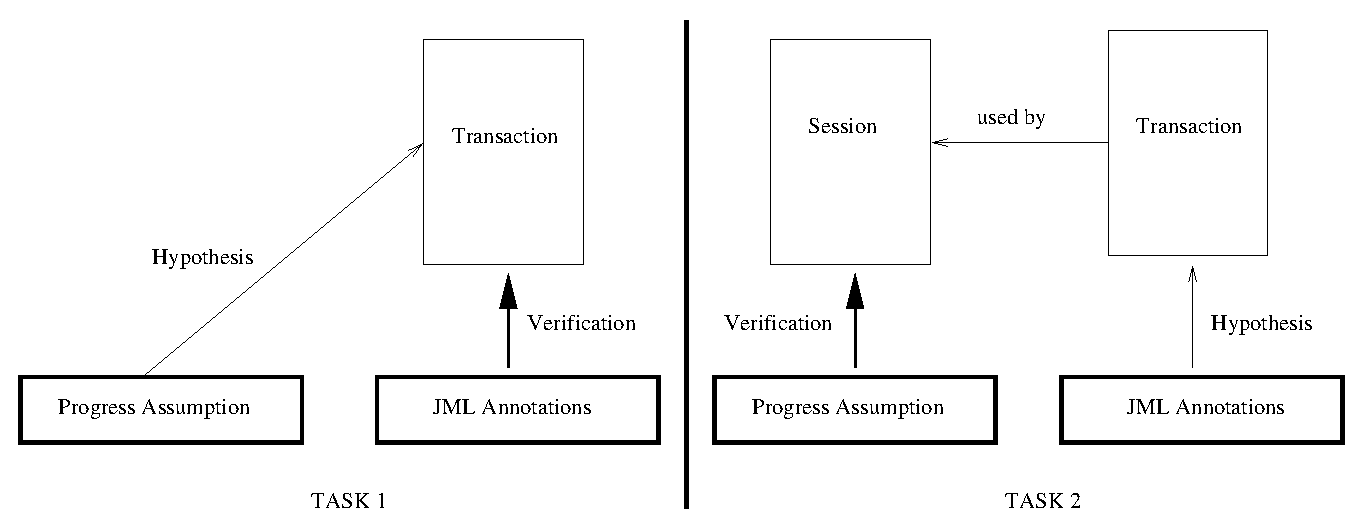
\includegraphics[scale=0.5]{model.eps}
\end{center}
\caption{Verification of Liveness Property: The example of Session and Transaction}

\label{fig-TS}
\end{figure}


%\begin{figure}[t]
%\begin{center}
%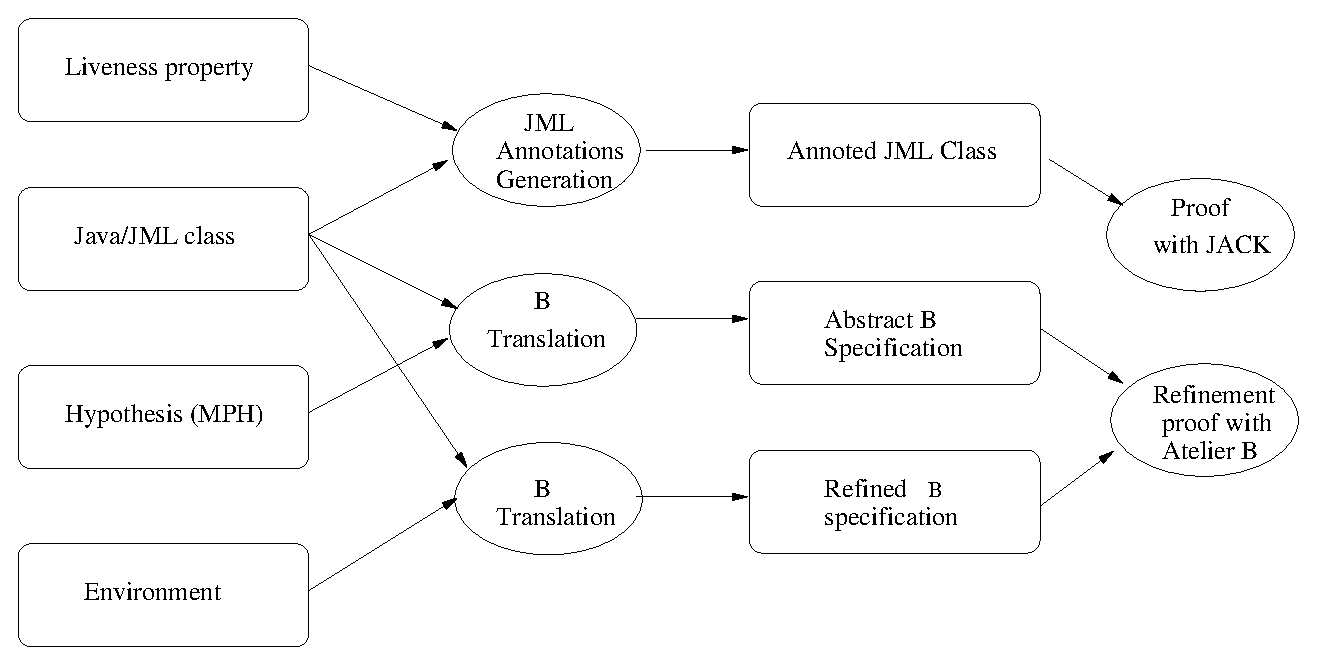
\includegraphics[scale=0.5]{general.eps}
%\end{center}
%\caption{Liveness Verification Method}

%\label{genpe}
%\end{figure}

%Indeed, the property ($L_F$)
%cannot be translated into an invariant.
 To prove a property expressed by the 
\textsf{Loop} operator on the class $Transaction$, 
one need to discover a \textit{variant} 
expression $V$ over a well-founded set. 
Under the condition $Q$,
$V$ must decrease each time a method of $Transaction$ terminates
until the $R$ happens.  %This expression $V$ is usually 
%called a variant. 
Moreover, the surrounding environment of the class, i.e., 
the class $Session$, must also verify some assumption. For example,
we are not able to prove the property ($L$), i.e., that the state 
\texttt{state == 6 || state == 7}
of the class $Transaction$ will eventually be reached, if the 
class $Session$ do not use any instance of $Transaction$. %For that, we need to asssume 
%some \textit{progress} on $Session$ to ensures the verification
%of the temporal property. 
So, to verify the liveness property ($L_F$), 
we need to assume \textit{progress}
on the environment of the class.

%The Figure~\ref{fig-TS} illustrate this problem.
Therefore, we divide the verification of the \textsf{Loop}
operator into two tasks as illustrated in Fig.~\ref{fig-TS}.




%This paper addresses this shortcoming by defining a way to verify
%liveness properties that can be expressed in this JML extension. 
%The basic idea of our approach is to break the verification into two
%different subtasks.  The Figure~\ref{fig-TS} illustrate this example.
\begin{itemize}
\item The first task is to show that, under a \textit{progress}
hypothesis on the environment $Session$, the property expressed by
the \textsf{Loop} operator is verified on the Java class 
$Transaction$, by generating appropriate
JML annotations. Particularly %, when
%$T$ is a liveness, 
one of 
these annotations guarantees that the methods of the class decrease
a variant $V$.  
%When $T$ is a liveness property,
%it is necessary to make some progress assumptions $H$ on the surrounding 
%class $Session$, in the case $T$ is a liveness property. Indeed, 

%Progress of the environment is needed for satisfaction 
%of the liveness properties,
% whereas it is not the case for a safety property. Indeed, according 
%to Lamport~\cite{Lamport77}, a class
%which is not used is always safe -- \textit{``something bad''} will never
%happen since nothing happens. However in general, it does not satisfy liveness %properties.
% Indeed nothing happens,  \textit{``something good''} will never happen.
%Therefore, for the verification of liveness properties, we need a progress 
%assumption $H$ on the environment, i.e., the class \textit{Session}, to 
%establish that $Transaction$ verify the liveness property $T$.

\item %The second task consists in verifying  that the 
%environment, i.e., the class $Session$, preserves the liveness 
%property $T$ when using $Transaction$, i.e., that $Session$
%verifies  the progress. Then $T$ is guaranteed on the whole
%system, i.e., the package $Session$ + $Transaction$.
The second task consists in verifying 
that the environment, i.e., the class $Session$, verify the
\textit{progress} hypothesis. Thus, the liveness property
will be verified on the whole system, i.e., $Transaction$ used by $Session$.
\end{itemize}



%The first subtask is to show that if the class
%\(transaction\) for
%which we wish to show the liveness property is run in an ideal
%environment, \emph{i.e.,}\/~an environment that calls all methods
%sufficiently often, then the liveness property can be established. 
%which  we wish to show the liveness property holds on a class used 
%by an environment under progress hypotheses $H$, then the liveness 
%property can be established. 
%The second subtask is to show that the surrounding system, in which the
%class \(C\) is actually used, preserves the liveness property. 


The paper is outlined as follows. Section~\ref{sec-RunningExample} 
presents JML and the running example.
Section~\ref{sec-temporal} explains liveness verification, 
and we show how to automatically generate JML annotations that are 
sufficient to guarantee liveness properties expressed by the
\textsf{Loop} operator,%defined in~\cite{Huis02},
assuming that the appropriate \textit{progress} assumptions holds on the
environment. We also prove the soundness of the generation.
We have implemented this annoation generation into a tool called \textsf{JAG}.
Section~\ref{sec-verif} presents the second task,
which requires to show that the environment satisfies the progress hypothesis.
The idea is to prove that the class and 
its environment is a liveness-preserving refinement of
the class \(C\) under the \textit{progress} assumption.  %Figure~\ref{genpe}
%depicts the general approach. Notice that instead of proving the JML
%annotations with JACK, they also could be validated using
%any other tool for JML.
Section~\ref{sec-conclusion} concludes and presents 
the perspectives of future work.





%\chapter{Java Validation}
This chapter gives an overview of the JML language and the tools that have been developed to deal with the it.

\section{Java and JavaCard}
 Formal validation of Java programs is a growing research
 field.  As Java has become a reference language, many technologies are
 emerging to help Java program validation.  Java can also be
 considered as a good support for formal techniques, as it has precise 
semantics \cite{Gosl00a}.

JavaCard is a popular programming language for multiple
application smart cards.  According to the JavaCard Forum \footnote{http://www.javacardforum.org},
which involves key players in the field of smart cards, 
including smart card manufacturers and banks, the JavaCard language has two
important features that make it the ideal choice for smart cards: 
\begin{itemize}
\item JavaCard programs are written in a subset of Java, using
the JavaCard APIs (Application Programming Interfaces). JavaCard
developers can therefore benefit from the well-established Java technology; 

\item the JavaCard security model enables multiple applications to
coexist  on the same card and communicate securely, and in principle,
enables new applications to be loaded on the card after its issuance.
\end{itemize}
Yet recent research has unveiled several problems in the JavaCard
security model, most notably with object sharing and the associated
mechanism of shareable interfaces.
This has  emphasized the necessity to develop environments for
verifying the security of the JavaCard platform and of JavaCard
programs.  Thus far JavaCard security (and also Java security) has
been studied  mainly at two levels:    
\begin{itemize}
\item  platform level: here the goal is to prove safety properties of
the language, in particular type safety and properties related to
memory management; 
\item  application level: here the goal is to prove that a specific
program obeys a given property, and in particular that it satisfies a
security policy, for example based on information flow. 
\end{itemize}
We are focusing at the application level, developing tools and methodologies based on JML to reach this goal.
\section{JML}
JML~\cite{Leavens-Baker-Ruby99b,Leavens-Baker-Ruby03}, the
``Java Modeling Language'', is a behavioral interface
specification language for Java; that is, it specifies both the behavior
and the syntactic interface of Java code.  The syntactic interface of
a Java class or interface consists of its method signatures,
the names and types of its fields, etc.
This is what is commonly meant by an application programming
interface (API).
The behavior of such an API can be precisely documented in JML annotations;
these describe the intended way that programmers should
use the API.  In terms of behavior, JML can detail, for example, the
preconditions and postconditions for methods as well as class
invariants.

An important goal for the design of JML is that it should be easily
understandable by Java programmers. This is achieved by staying as
close as possible to Java syntax and semantics.  Another important
design goal is that JML {\em not} impose any particular design method
on users; instead, JML should be able to document Java programs
designed in any manner \cite{Leavens-Baker-Ruby03}.

JML uses Java's expression syntax in assertions,
thus JML's notation is easy for programmers to learn.  
Because JML supports quantifiers such as
\verb_\forall_ and \verb_\exists_, and because JML allows ``model''
(i.e., specification-only) fields and methods, specifications can
easily be made precise and complete.
JML assertions are written as special
annotation comments in Java code,
so that they are ignored by Java compilers but can be used
by tools that support JML\@.  Within annotation comments JML extends the
Java syntax with several keywords.  It also extends Java's expression syntax with several
operators.
The central ingredients of a JML specification are preconditions
(given in {\tt requires} clauses), postconditions (given in {\tt
  ensures} clauses), and (class and interface) invariants.  These are
all expressed as boolean expressions in JML's extension to Java's
expression syntax.
In addition to ``normal'' postconditions, the language also supports
``exceptional'' postconditions, specified in {\tt signals} clauses.
These can be used to specify what must be true when a method throws an
exception. 

%=====================================================================
%=====================================================================
\subsection{The JML tool suite}
\label{tools}

Since JML specifications are meant to be read and written by ordinary
Java programmers, it is important to support the conventional ways
that these programmers create and use documentation.  Consequently,
the {\tt jmldoc} tool
produces browsable HTML pages containing both the
API and the specifications for Java code, in the style of pages
generated by Javadoc~\cite{Friendly95}.

%=====================================================================
The JML compiler (\texttt{jmlc}), developed at Iowa State University,
is an extension to a Java compiler and compiles Java programs
annotated with JML specifications into Java
bytecode~\cite{Cheon03,Cheon-Leavens02b}.  The compiled bytecode includes
runtime assertion checking instructions that check JML specifications
such as preconditions, normal and exceptional postconditions,
invariants, and history constraints.  The execution of such assertion
checks is transparent in that, unless an assertion is violated, and
except for performance measures (time and space), the behavior of the
original program is unchanged.  The transparency of runtime assertion
checking is guaranteed, as JML assertions are not allowed to have any
side-effects~\cite{Leavens-etal03a}.




\section{ESC/Java2}
\label{escjava}

ESC/Java2 tool~\cite{Flanagan-Et-Al02}, originally developed at Compaq Research,
performs what is called ``extended static
checking''~\cite{ESC:Overview,10yearsESC},
compile-time checking that goes well beyond type checking.  It can
check relatively simple assertions and can check for certain kinds of
common errors in Java code, such as dereferencing \texttt{null},
indexing an array outside its bounds, or casting a reference to an
impermissible type.  ESC/Java2 supports a subset of JML and also checks
the consistency between the code and the given JML annotations.  The
user's interaction with ESC/Java2 is quite similar to the interaction
with the compiler's type checker: the user includes JML annotations in
the code and runs the tool, and the tool responds with a list of
possible errors in the program.

JML annotations affect ESC/Java2 in two ways.  First, the given JML
annotations help ESC/Java2 suppress spurious warning messages.   Second,
annotations make ESC/\-Java2 do additional checks.  
In these two ways, the use of JML annotations enables ESC/Java2 to
produce warnings not at the source locations where errors manifest
themselves at runtime, but at the source locations where the errors
are committed.

%=====================================================================
%\section{Applications of JML to Java Card}
%\label{applications}

%Although JML is able to specify arbitrary sequential Java programs,
%most of the serious applications of JML and JML tools up to now
%have targeted Java Card.  Java Card$^{TM}$ is a dialect of Java specifically
%designed for the programming of the latest generation of smartcards.
%Java Card is adapted to the hardware limitations of smartcards; for
%instance, it does not support floating point numbers, strings, object
%cloning, or threads.

%Java Card is a well-suited target for the application of formal
%methods.  It is a relatively simple language with a restricted API\@.
%Moreover, Java Card programs, called ``applets'', are small, typically
%on the order of several KBytes of bytecode.  Additionally, correctness
%of Java Card programs is of crucial importance, since they are used in
%sensitive applications such as bank cards and mobile phone SIMs.  (An
%interesting overview of security properties that are relevant for Java
%Card applications is available~\cite{MarletLM01}.)

%JML, and several tools for JML, have been used for Java Card,
%especially in the context of the EU-supported project VerifiCard
%(www.verificard.org).  JML has been used to write a formal
%specification of almost the entire Java Card
%API~\cite{PollBergJacobs01}.  This experience has shown that JML is
%expressive enough to specify a non-trivial existing API\@.  The
%runtime assertion checker has been used to specify and verify a
%component of a smartcard operating system~\cite{PollHarteldeJong02}.





\section{Introduction to JML on a Example}
\label{sec-RunningExample}


\begin{floatingfigure}[l]{6cm}
\begin{center}
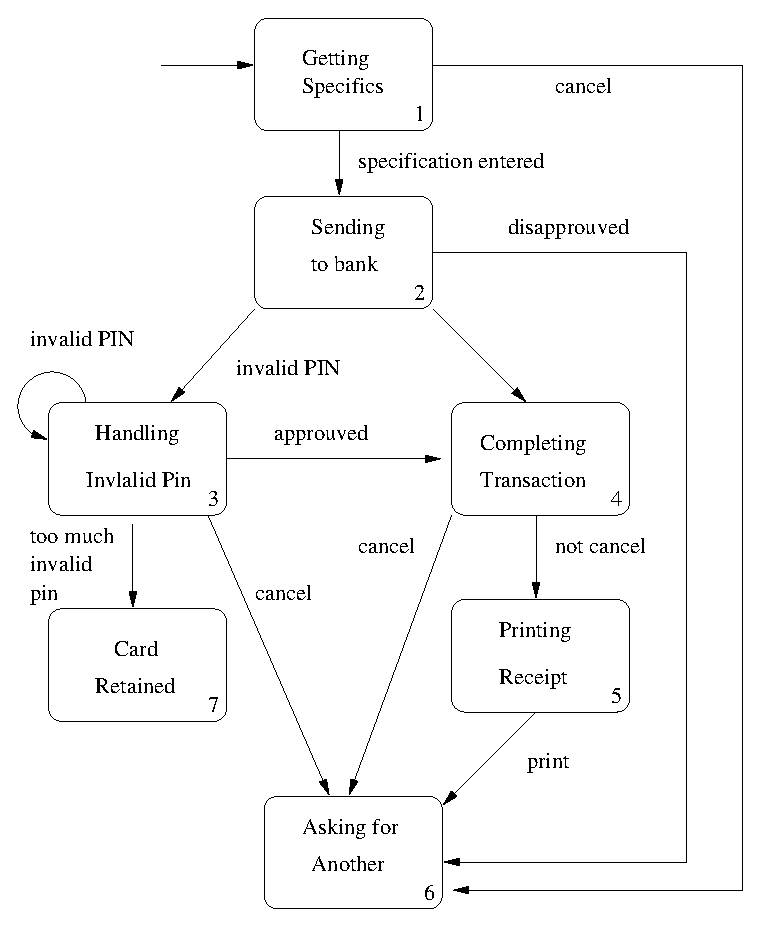
\includegraphics[scale=0.4]{Transac.eps}
\end{center}
\caption{Transaction System Graph}
\label{fig-Transac}
\end{floatingfigure}
The transaction mechanism of 
the ATM specification (see Sect.~\ref{SecIntro}) 
was initially designed by a 
 diagram (see Fig.~\ref{fig-Transac}). It works as follows.
First, when a transaction is initialized, it get information
from the customer (amount, type of transaction...). Second,
this information is sent to the bank, which may approve 
or disapprove the transaction (amount too high for the account...).
In the case of approval, and if the PIN code is confirmed, the
transaction can be completed. Otherwise the PIN code is asked again
until the PIN limit (normally only three at\-tem\-pts are authorized). When
the PIN lim\-it is reached, the card is retained. 
After a transaction completion, the customer may obtain a ticket. 
At each step, it is possible to cancel the transaction.
%We would like to implement this transaction system. 
This transaction system is implemented by a Java Class $Transaction$.
We have 
described this class, according to the diagram (see Fig.~\ref{fig-Transac})
using JML specifications (Fig.~\ref{FigRunningExample}).
JML (Java Modeling
Language)~\cite{Leavens-etal03} is a specification
language especially tailored for Java applications. Originally, JML
was proposed by G.T.~Lea\-vens and his team; nowadays the development of
JML is a community effort. JML has been successfully used in several
case studies to specify Java applications, and notably to specify
smart card applications, written in Java
Card~\cite{BreunesseCHJ03,BousquetLMOL04,JacobsMR04}.



%%%%%%%%%%%%%%%%%%%%%%%%%%%%%%%%%%%%%%%%%%%%%%%%%%%%%%%%%%%
%JML introduce its own  variables. 
%These exist also only in specifications, but a special
%\texttt{set} annotation exists to change their value.% (while
%\texttt{model} variables change implicitly, when the concrete
%variables they represent change).
%F%urther 
The reader can see a declaration of a class \texttt{invariant}, denoting a
predicate that has to hold before and after every method call.  We can also
specify history \texttt{constraint}s, expressing a relation between the
pre- and post-state of a method. Pre-state values of expressions are
denoted by the JML keyword \texttt{$\backslash$old}. Moreover, one can
specify, using the clause \texttt{for}, the list of the methods on which
the history constraint must be verified. When this clause is omitted, the
constraint must hold on all the methods of the class.  Finally, behavior of
the methods can be specified using keyword \texttt{normal\_behavior}. The
clause \texttt{requires} denotes the precondition of the method, i.e.  a
predicate that must be true when the method is called. We can also specify
postcondition (\texttt{ensures} clause).  A method can terminate
exceptionally, by throwing an exception and satisfying the exceptional
postcondition (\texttt{signals} clause). In this case, we have a
\texttt{behavior} specification. The validation of this model can be done
using JML-TT-Animator, a symbolic animator for JML
specification~\cite{bdlu05}. The faithfulness of the JML model w.r.t. the
Java code is done by a prover (B or Coq) via a proof
obligations generator (Jack or Krakatoa). 
 


In the rest of the paper, given the JML model of a class $C$, we denote 
\(\mathcal{P}red_C\) the set of the JML predicates.




% \marginpar{ajouter
% que la conformité à la spec n'est pas une garantie: faut-il encore que la spec n'ait pas de faille.}




\begin{figure}[h]
\begin{multicols}{2}
\begin{scriptsize}
\ttfamily

            private int state = 1;\\
            private static  int PIN\_MAX\_TRY = 3;\\
            private int pin\_try = 0;\\
           /*@ invariant state $>$= 1 \&\&\\
           ~~@ state $<$ 8;\\
           ~~@*/


            /*@ private normal\_behavior\\
~\quad         @ requires state == 1;\\
~\quad         @ modifies state;\\
~\quad         @ ensures  state == 2 \\
~\quad         @     ||  state == 6;\\
~\quad         @*/\\
            private void initialiseTransaction()\{...\}\\
           
            /*@ private  normal\_behavior\\
\quad         @ requires state == 2 ;\\
\quad         @ modifies state,pin\_try,pin\_validated;\\
\quad         @ ensures  (state == 3 \\
\quad         @ \qquad                \&\& pin\_try == $\backslash$old(pin\_try) + 1\\
\quad         @ \qquad                \&\& pin\_validated == false) \\
\quad         @ \quad     ||   (state == 6 \\
\quad         @ \qquad                \&\& pin\_try == $\backslash$old(pin\_try)\\
\quad         @ \qquad               \&\& pin\_validated == false)\\
\quad         @ \quad    ||   (state == 4 \\
\quad         @ \qquad               \&\& pin\_try == $\backslash$old(pin\_try)\\
\quad         @ \qquad               \&\& pin\_validated == true);\\
\quad         @*/\\
            private void sendToBank()\{... \}\\
            
            /*@ private behavior\\
\quad         @ requires state == 3;\\
\quad         @ modifies state,pin\_try,pin\_validated;\\
\quad         @ ensures (state == 4)\\
\quad         @  \quad     || (state == 6\\
\quad         @  \qquad         \&\& pin\_try == $\backslash$old(pin\_try)\\
\quad         @  \qquad         \&\& pin\_validated == true\\
\quad         @  \qquad         );\\
\quad         @ signals (Exception) (state == 7 \\
\quad         @  \qquad        \&\& pin\_try == PIN\_MAX\_TRY\\
\quad         @  \qquad        \&\& pin\_try == $\backslash$old(pin\_try) + 1\\
\quad         @  \qquad        \&\& pin\_validated == false);\\
\quad         @ signals (Exception) (state == 3 \\
\quad         @  \qquad        \&\& pin\_try < PIN\_MAX\_TRY\\
\quad         @  \qquad        \&\& pin\_try == $\backslash$old(pin\_try) + 1\\
\quad         @  \qquad        \&\& pin\_validated == false);\\
\quad         @*/\\
            private void pinValidation() \{... \}\\
            
            
            /*@ private  normal\_behavior\\
\quad         @ requires state == 4;\\
\quad         @ modifies state;\\
\quad         @ ensures state == 5\\
\quad         @ \qquad      || state == 6;\\
\quad         @*/\\
            private void complete()\{...\}\\
            
            
            /*@ private  normal\_behavior\\
\quad         @ requires state == 5;\\
\quad         @ modifies state;\\
\quad         @ ensures state == 6;\\
\quad         @*/\\
            private void printReceipt()\{ ... \}\\

 /*@ private  normal\_behavior\\
\quad  @ ensures $\backslash$result ==  (PIN\_MAX\_TRY - pin\_try);\\
\quad         @*/\\
public void /* pure */ getTryLess()\{...\}
          

\normalfont
\setlength{\parindent}{1cm}
\end{scriptsize}
\end{multicols}
\caption{Transaction System Example}
\label{FigRunningExample}


\end{figure}






%%% Local Variables: 
%%% mode: latex
%%% TeX-master: "main2"
%%% End: 


 \section{Verification of Liveness Properties using a \textsf{Loop} primitive}\label{sec-temporal}

%In earlier work, Trentelman and Huisman~\cite{Huis02} propose an
%extension of JML with temporal logic constructs especially dedicated
%%to the semantics of Java and inspired by the
%\emph{Specification Patterns} developed by Dwyer \emph{et
%al.}~\cite{1999:icse:dwyer}. We use this language as a basis
% for our
%work, but we extend it by requiring the additional
% specification of a
%variant and an invariant for liveness
% properties. Variants and Invariants are used to
%prove the validity of the formulae, as described in Section~\ref{sec-until}.
%Below, in Section~\ref{sec-until} we will show how this
%variant and invariant are used to prove that an application satisfies
%these liveness properties.

%In this section we present the formal model underlying 
%the semantics of the language, the trace-based semantics of the language 
%itself, and how we extends it for the verification of liveness
%properties.


%(informal) syntax and semantics of this
%extension, and we discuss how we add the notions of variant and
%invariant to the specification of the liveness properties.

This section deals with the verification of a liveness 
properties expressed by a \textsf{Loop} primitive as 
follows. This section is outlined as follows. 
Section~\ref{sec:prelim} presents the formal execution model,
Section~\ref{sec-until} presents the \textsf{Loop} primitive and a
progress hypothesis on the environment that ensures the 
satisfaction of the \textsf{Loop} primitive. The translation
of the \textsf{Loop} operator into standard \textsf{JML}
assertions is given in \ref{sec-OPLoop}. Section~\ref{sec-env} presents
a progress hypothesis on the environment ($PH$) which
is shown to be %minimal, i.e., 
necessary and sufficient to
ensure the satisfaction of the liveness property.


\subsection{Formal Execution Model}
\label{sec:prelim}

%In the next subsection, we give the formal semantics of the JML extension 
%with temporal specifications. 
This section  describes the formal model we use, 
based on transition systems.
%To verify liveness properties expressed by the \textsf{loop} operator, 
%we only need to observe the
%methods that modify the internal states of the class, 
%and so we abstract the others into a \textit{skip event}. 
%This abstraction allows us 
%to reason more easier about Java program execution.

\begin{definition}[Progress and Non-progress Methods]
  Given a class $C$, we distinguish the set of all the methods with
  side-effect, i.e., that may modify the value of the attributes of $C$. We
  call these methods \emph{progress methods} of $C$, denoted by
  $\mathcal{PM_C}$. The other methods (\emph{getters} of $C$) are in
  $\overline{\mathcal{PM_C}}$
 
%Given a class $C$, a method $m$ is called an observer if the execution of $m$
%does not modify the value of the variable of $C$, otherwise, i.e.,
%if the execution of $m$ may affect the value of the variables of 
%class $C$, then $m$ is a progress method.
\end{definition}

%\begin{definition}[Skip Event]
%Each call or termination of a observer method is denoted as a skip event. 
%\end{definition}
%By definition, each call to an observer method of the class or an external 
%method is seen as a skip event. 



%By definition, each call or termination of an observer method of the class
%can be seen as a \textit{skip} event.




%The temporal logic language  is defined over a trace semantics, 
%so we introduce transition systems as a
%% formal notion of system and execution.

The \textsf{Loop} primitive is defined over an execution.  So, we introduce
transition systems as a formal model of an environment using the class
methods. It reflects a semantics of calls and terminations
of the methods of the class $C$ in an environment respecting $PH$. % notion of system and execution.

\begin{definition}[Transition System]\label{def-TS}   
Let $Ev$ be a nonempty alphabet of
\emph{events} and \(\mathcal{P}red_C\) a set of JML predicates
over the variables of a class $C$.
A interpreted \emph{transition system} $TS_C$ is a tuple
$<S,S_0,\rightarrow,l_C>$ composed of 
a set of states \(S\), 
a set of initial states $S_0\subseteq S$, 
a total transition relation $\rightarrow{} 
\subseteq S \times S$, 
and a state interpretation function $l_C$ : $S \rightarrow
\mathcal{P}(\mathcal{P}red_C)$. 
\end{definition}

The semantics of \textsf{Loop} is defined over infinite sequences of states
(executions) of a transition system.
\begin{definition}[Execution]
\label{def-TSexec}
Given a transition system \(TS_C = <S, S_0, \rightarrow, l_C>\), an
\emph{execution} $\sigma$  of $TS_C$ is an infinite sequence
$s_0, s_1, s_2, \ldots , s_i, s_{i+1}, \ldots$ of
states such that $s_0 \in S_0$ 
and for each $i \ge 0$, $(s_i \xrightarrow{} s_{i+1}) \in \rightarrow$. 
We denote $\Sigma_C$ the set of all the executions of $TS_C$.
\end{definition}
For any JML predicate \(P \in\mathcal{P}red_C\), and any state \(s \in
S\), we say that $s$ satisfies $P$, written \(s\sat P\) 
whenever \(P \in l_C(s)\). 
A JML predicate \(P\) holds on an execution \(\sigma\), denoted \(\sigma
\sat P\), if \(s_0 \sat P\).
We have also to define the conformity of an execution $\sigma$
with respect to a set of JML annotations $\mathcal{A}$ of a class $C$,
written $\sigma : \mathcal{A}$. It can be extended to all the executions
from $\Sigma_C$ ($\Sigma_C :  \mathcal{A}$), or to the transition system
$TS_C$ ($TS_C : \mathcal{A}$).  
% To define the  semantics, we also define
%e%xecution suffixes and segments.
 
\begin{definition}[Execution suffix]
Given an execution \(\sigma\), the \emph{execution suffix} beginning
at the index $i$, denoted \(\sigma_i\), is the infinite sequence
\[ s_i , s_{i+1} , s_{i+2}, \ldots \]

%{\noindent
%Given an execution $\sigma$, the \emph{execution segment} \(\sigma^j_i\)
%denotes the infinite sequence
%}
%$$ s_i \xrightarrow{e_{i+1}}s_{i+1}
% \ldots s_{j-1} \xrightarrow{e_j} s_{j} \xrightarrow{skip} s_j \ldots $$
\end{definition}

We say that \(P\) holds on \(\sigma_i\) %and \(\sigma_i^j\) 
if \(s_i \sat P\). 
%Finally, we formally define what we mean be occurrence of an event in \(E\).
%\begin{definition}[Occurrence of events]
%\label{def-E-hold} 
%Let \(E \subseteq Ev\) be a set of events and \(\sigma\) an execution.
%We say an event in
%\(E\) \emph{occurs} in state $s_i$, written $s_i \models E$,
%if \(e_{i} \in E\).




 %\(e_{i}\) is called a \emph{\(E\)-transition}.
%We call the transition \(s_{i} \xrightarrow{e_{i+1}} s_{i+1}\) an
%\emph{\(E\)-transition}. 



%We say an event \(e\) \emph{occurs} on \(\sigma\) if there exists an \(i\)
%such that \(s_i \sat e\). 
%We say an event \(e\) does \emph{not occur}
%on \(\sigma\) if for all \(i\) we have \(s_i \not\sat e\). 
%\end{definition}


%\begin{definition}[Progress of an Execution]
%Let $\sigma$ be an infinite execution over a transition system,
%we say that $\sigma$ progresses for all states $s$ of the
%execution if there exists a state $s'$ in the future such that 
%$l(s)$ is not equivalent to  $l(s')$.
%\end{definition}


%%% Local Variables: 
%%% mode: latex
%%% TeX-master: "main2"
%%% End: 



\subsection{The \textsf{Loop} Primitive and the Main Theorem}% and a Sufficient Hypothesis on the Environment}
\label{sec-until}

%To generate JML annotations for liveness properties, 
This section introduces
the  \textsf{Loop} primitive \(Q \leadsto_{\mathit{JML}} R (J,V,M)\), 
the sufficient progress hypothesis $H_{S_1}$ on the environment, and the
main theorem for generating annotations that conform the \textsf{Loop}
primitive. 

%\subsubsection{The \textsf{Loop} primitive}
\begin{definition}[\textsf{Loop} Primitive]\label{until1} 
  Let \(R\), \(Q\) and \(J\) be in $\mathcal{P}red_C$, \(M\) a subset of
  the progress methods $\mathcal{PM}_C$, and \(V\) a JML expression
  returning an integer.  The \textsf{Loop} primitive \(Q
  \leadsto_{\mathit{JML}} R 
  (J,V,M)\) holds on the execution $\sigma$, written $\sigma \models Q
  \leadsto_{\mathit{JML}} R (J,V,M)$, if
\[
\forall i. (i \geq 0
\wedge \sigma_i \models Q ) ~
\Rightarrow ~ (\exists j. j > i \wedge \sigma_j \models R \wedge
~(\forall k.i \leq k<j \Rightarrow \sigma_k \models Q )).
\]
\end{definition}
%Notice that implicitly \(\sigma\) is supposed to satisfy the
%hypotheses described in Sect.~\ref{sec-until-environment}, thus
%calling the methods in \(M\) infinitely often. 
Notice that the
invariant \(J\) and the variant $V$ do not appear in the above
expression,%this definition, 
they are only used to generate the appropriate proof obligations for
the termination of the loop.\\


%We now describe an Hypothesis ($H_S$) on the surrounding environment 
%-- in our example, the
%class $Section$ -- which is sufficient to permit the verification of liveness 
%properties using JML annotations.%, i.e., which permits to have infinite
%executions.

%Second, assuming that the environment verifies this hypothesis, we
%give the needed JML annotations to verify the liveness property.
%Section~\ref{sec-verif} discusses how the
%assumptions on the environment can be verified.

%Remember that for the time being, we assume all methods in \(C\) to be atomic,
%\emph{i.e.,}\/~they do not call any other method.





%\subsubsection{Hypothesis on the Environment}



%Let $M$ be the set of all non-observer methods of $C$, 
%assuming that we verify a liveness property expressed by the 
%operator $Q \leadsto R (J,V,M)$



Contrarily to safety properties, it is not possible to verify liveness
properties without information about the programs, that use 
the class. 

We propose a hypothesis $H_{S_1}$ on the environment which is sufficient to
guarantee a liveness property when some JML annotations are faithful w.r.t.
the class methods. The hypothesis $H_{S_1}$ requires that the environment
calls a progress method of the class infinitely often.  The hypothesis
($H_{S_1}$) can be expressed in the semantics of LTL~\cite{pnueli77}, using
the $F^{\infty}$ operator. % (see Appendix~\ref{appendix-PLTL}). 
Given a predicate $P$, the formula $F^{\infty} P$  
means that $P$ occurs \textit{``infinitely often''}, i.e., for each state
of the execution, there exists a future state verifying $P$. Formally,
$$\sigma_i \models F^{\infty} P \equiv_{def} \forall j \geq i . (\exists k
. ( k\geq j \wedge \sigma_k \models P))$$

$H_{S_1}$ can be expressed as follows.

$$ \hspace*{15em} (\mathsf{F^{\infty}} M ~ \mathbf{called})
  \hspace*{11em} (H_{S_1})$$

%Where $M$ denotes the set of non-observer methods of the class
%and  $M$ \textbf{called} denotes the predicate 
%$\bigvee_{m \in M} m ~ \mathbf{called}$.

where  $(M ~ \mathbf{called})$ is a predicate denoting 
that a progress method of the class has been called.



Assuming that the environment satisfies $H_{S_1}$, we are able to give JML
annotations that ensure the satisfaction of a liveness property on a given
execution. This is the matter of Sections~\ref{sec-OPLoop}.






%It means that if \emph{Q} holds on a state of the execution $\sigma$,
%in the future we eventually have a state which satisfies \emph{P} (in
%the following \emph{Q} is always a predicate which is satisfied until
%\emph{P} holds, so we call this modality a \emph{Until} modality).


\subsection{Main Theorem}%Proof Obligation of the \textsf{Loop} primitive}
\label{sec-OPLoop}

We give the proof
obligations inspired from~\cite{Abrial:1998:IDC,burstall}, and expressed as
JML annotations. The proof obligations guarantee 
the satisfaction of the \textsf{Loop}
primitive under the hypothesis $H_{S_1}$. 


Let \(Q \leadsto_{\mathit{JML}} R (J, V, M)\) be the \textsf{Loop}
primitive. Let $\mathcal{A}_{1-6}$ be the following set of JML annotations. 


\begin{small}
\begin{enumerate}
\item \emph{\texttt{//@ invariant} \(Q\) \texttt{==>} \(J\);}

\item \emph{\texttt{//@ invariant} \(V\) \texttt{>= 0};}

\item \emph{\texttt{//@ constraint \bsl old(}\(Q\)\texttt{) \& \bsl
old(}\(J\)\texttt{) \& !}\(R\) \texttt{\:==>\:} Q \texttt{
for} \(M\);}
\item \emph{\texttt{//@ constraint \bsl old(}\(Q\)\texttt{) \& \bsl
old(}\(J\)\texttt{) \& !}\(R\) \texttt{\:==>\:} \(V\) \texttt{< \bsl old(}\(V\)\texttt{)
for} \(M\);}

\item \emph{\texttt{//@ constraint \bsl old(}\(Q\)\texttt{) \& \bsl
old(}\(J\)\texttt{) \& !}\(R\) \texttt{\:==>\:} \(V\) \texttt{<= \bsl
old(}\(V\)\texttt{) for} \(\overline{M}\);}

\item \emph{\texttt{//@ constraint \bsl old(}\(Q\)\texttt{) \& \bsl 
old(}\(J\)\texttt{)  \& !}\(R\) \texttt{\:==>\:}   \(\exists m.\:  
m\in \mathcal{PM_C}\)} %%%\mathsf{requires}(m)\) \texttt{\&} \(\neg \mathsf{diverges}(m)\);}
\end{enumerate}
\end{small}
\marginpar{pb with OP6 JG}.


The meta-notation (\(\exists m.\: \mathsf{requires}(m)\) \texttt{\&} \(\neg
\mathsf{diverges}(m)\) ) is not a JML property. This can be written in JML
as the negation of the predicate of the \texttt{diverges} clause and the
disjunction of all the method's preconditions.
%\marginpar{a modifier version journal}



\begin{theorem}[Main Theorem]%JML Annotations for the \textit{Loop}]
  \label{until} 
If $\Sigma_C : \mathcal{A}_{1-6}$ and $\Sigma_C \models H_{S_1}$ then 
$\Sigma_C \models Q \leadsto R (J,V,M)$. 
%\begin{center}
%\begin{tabular}{c}
% $\Sigma_C : \mathcal{A}_{1-6}$\\
% $\Sigma_C \models H_{S_1}$\\
% \hline
% $\Sigma_C \models Q \leadsto R (J,V,M)$\\
% \end{tabular}
% \end{center}
\end{theorem}

In other words, assuming that an execution $\sigma$ in $\Sigma_C$ of the
environment of a class $C$ satisfies $H_{S_1}$, \(Q
\leadsto_{\mathit{JML}} R (J, V, M)\) holds on $\sigma$ if $\sigma :
\mathcal{A}_{1-6}$.

%the following proof obligations are satisfied%\:\footnote{where
%\(\mathsf{term}(M)\) is the set of events 
%\(\{ m~\mathbf{terminates}, m~\mathbf{exceptional}, m~\mathbf{normal} \mid m \in M\}\), 
%\(\mathsf{requires}(m)\)  denotes the precondition, and
%\(\mathsf{diverges}(m)\) the diverges
%clause --the conditions under which the method might
%diverge --, of method \(m\), respectively.}.


%\begin{footnotesize}
%\begin{gather}
%\forall i.\:(\sigma_i \models  Q ) \Rightarrow ( \sigma_i \models J ) \\
%\forall i.\:\sigma_i \models (V \in \mathbb{N})\\
%\forall i\:, n.\:(\sigma_i \models  (Q \wedge J \wedge V = n) \Rightarrow
%((\sigma_{i+1} \models \neg  R \wedge \mathsf{term}(M))
%%\wedge \sigma_i \models V = n \wedge \sigma_i \models event(M)
%\Rightarrow \sigma_{i+1} \models Q))\\
%\forall i\:, n.\:(\sigma_i \models  (Q \wedge J \wedge V = n) \Rightarrow
%((\sigma_{i+1} \models \neg  R \wedge \mathsf{term}(M))
%%\wedge \sigma_i \models V = n \wedge \sigma_i \models event(M)
%\Rightarrow \sigma_{i+1} \models V < n))\\
%\forall i\:, n.\:(\sigma_i \models  (Q \wedge J \wedge V = n)
%\Rightarrow
%((\sigma_{i+1} \models \neg  R \wedge \mathsf{term}(\overline{M})) 
%%\wedge \sigma_i \models V = n \wedge \sigma_i \models
%%event(\overline{M}) 
%\Rightarrow \sigma_{i+1} \models V \leq n))\\
%\forall i.\:(\sigma_i \models (Q \wedge J) 
%%~ \wedge ~ \sigma_i \models J  ~\wedge ~ 
%\Rightarrow (\sigma_{i+1} \models \neg  R ~ \Rightarrow  
%(\exists m.\:\sigma_{i+1} \models (\mathsf{requires}(m) \wedge \neg \mathsf{diverges}(m)))))
%\end{gather}
%\end{footnotesize}



%Notice that these JML annotations, 
%completed by Hypothesis~($H_{S_1}$), basically describe a
%termination proof~\cite{}:%, using an invariant
% $J$ and a variant $V$, from which we
%can conclude that eventually \(R\) should hold. 
Intuitively, $\mathcal{A}_{1-6}$ could be understood as follows.
\begin{enumerate}
\item The invariant \(J\) has to hold, whenever \(Q\) holds.
\item The variant $V$ actually expresses a natural number,
\emph{i.e.,}\/~it is well-founded.
\item %If $Q$ holds in the preceeding state, and $R$ do not 
%hold in the current state, then $Q$ must holds in the 
%current state. 
The predicate $Q$ is preserved unless $R$ holds on the current state.
\item If \(Q\) holds, and a method in $M$ is called, the variant \(V\) must
  strictly decrease. It ensures the progress when the environement satifies
  $H_{S_1}$ (livelock-freeness).
\item If \(Q\) holds, and a method in $\overline{M}$ is
  called, the variant \(V\) may not increase.
%After a state where Q holds, the variant $V$ must decrease after
%each event until the predicate P is satisfied. This proof obligation
%establishes that we have no livelock in Q.
%\item We have to prove that all the observer methods (methods that
%belongs to the complementary set of $M$ denoted $\overline{M}$) must
%not increase the variant $V$

\item As long as \(Q\) holds, and \(R\) is not reached, there always
should be a method enabled (\emph{i.e.,}\/~its precondition holds, and
it will not diverge). This ensures the deadlock-freeness of the system.

%We have to ensure, that after a state where Q holds, the system
%cannot be blocked until the state where P holds. To do that, we verify
%for each of these states, that at least one precondition of a method
%is true (that means, that at least one method can be invocated), and
%we have to verify that if the method holds then this method cannot
%diverge.
\end{enumerate}
The reader can find a formal expression of $\mathcal{A}_{1-6}$) in
Lemma~\ref{lemma-loop}. The proof of the main theorem is given in
Appendix~\ref{sec-proof-theorem-loop}.







%Following Theorem~\ref{until} and the JML
%semantics~\cite{TheseMarieke}, the following JML annotations are
%sufficient to imply the validity of the
%\emph{Loop} primitive.


%\begin{proposition}[JML Proof Obligations \emph{Loop}]\label{PropLeadsTo}
%The following JML assertions implies that
%$Q\leadsto_{\mathit{JML}}R(J,V,M)$ holds. 

%\end{proposition}
%\marginpar{commentaires ???}
%The first and second proof obligations are simply expressed in
%JML by an invariant. We other,




%The generation of JML annotations that ensure liveness properties 
%in JML is done through this $Loop$ primitive. Next subsection shows
%the appropriate annotations for the liveness
%property ($L_C$).


%%% Local Variables: 
%%% mode: latex
%%% TeX-master: "main2"
%%% End: 


%%\subsection{Application to the Example}\label{sec-casestudy}



%\begin{figure}[hp]
%
%\begin{multicols}{2}
%\begin{scriptsize}
%\ttfamily
%
%	    private int state = GETTING\_SPECIFICS\_STATE;\\
%	    private static  int GETTING\_SPECIFICS\_STATE = 1;\\
%	    private static  int SENDING\_TO\_BANK\_STATE = 2;\\
%	    private static  int INVALID\_PIN\_STATE = 3;\\
%	    private static  int COMPLETING\_TRANSACTION\_STATE = 4;\\
%	    private static  int PRINTING\_RECEIPT\_STATE = 5;\\
%	    private static  int ASKING\_DO\_ANOTHER\_STATE = 6;\\
%	    private static  int CARD\_RETAINED\_STATE = 7;\\
%	    private static  int PIN\_MAX\_TRY = 3;\\
%	    private int pin\_try = 0;\\
%	    private boolean pin\_validated = false;\\
%\begin{tabular}{|l|}
%\hline
%/*@ ghost bool Pa =\\
%\quad @ (state == 7 || state == 6);\\
%\quad @*/\\
%\hline
%\end{tabular}

%\begin{tabular}{|l|}
%\hline
%//@ ghost bool Pe = pin\_validated;\\
%\hline
%\end{tabular}


%\begin{tabular}{|l|}
%\hline
%/*@ ghost bool complete\_called\\
%\quad @ = pin\_validated;\\
%\quad @*/\\
%\hline
%\end{tabular}



%\begin{tabular}{|l|}
%\hline	    
%//@ invariant complete\_called =$>$ Pe;\\
%\hline
%\end{tabular}\\




%\begin{tabular}{|l|}
%\hline	    
%//@ invariant true =$>$ true;\\
%\\
%/*@ invariant ((7 - state) + \\
%\quad @ \quad getTryLess()) $>$ 0;\\
%\quad @*/\\
%\\
%/*@ constraint $\backslash$old(!Pa) \\
%\quad @ \quad \&\& !(state == 7 || state == 6) =$>$ \\
%\quad @ (7 - state + getTryLess()) \\
%\quad @ \quad $<$ $\backslash$old(7 - state + getTryLess())\\
%\quad @ for initialiseTransaction, sendToBank, \\
%\quad @ pinValidation, complete,   printReceipt;\\
%\quad @*/ \\ 
%\\
%/*@ constraint $\backslash$old(!Pa) \\
%\quad @ \quad \&\& !(state == 7 || state == 6) =$>$ \\
%\quad @ (7 - state + getTryLess()) \\
%\quad @ \quad $<$= $\backslash$old(7 - state + getTryLess())\\
%\quad @ for getTryLess;\\
%\quad @*/ \\ 
%\\
%/*@ constraint $\backslash$old(!Pa) \\
%\quad @ \quad \&\& !(state == 7 || state == 6) =$>$ \\
%\quad @ ( state == GETTING\_SPECIFICS\_STATE\\
%\quad @ || state == SENDING\_TO\_BANK\_STATE\\
%\quad @ || state == INVALID\_PIN\_STATE;\\
%\quad @ ||state == COMPLETING\_TRANSACTION\_STATE\\
%\quad @ || state == PRINTING\_RECEIPT\_STATE;)\\
%\quad @*/ \\ 
%\hline

 
%\end{tabular}
%\\


%	    /*@ private behaviour\\
%\quad	      @ requires state == GETTING\_SPECIFICS\_STATE;\\
%\quad	      @ modifies state;\\
%\quad	      @ ensures  state == SENDING\_TO\_BANK\_STATE \\
%\quad	      @ \qquad    ||  state ==ASKING\_DO\_ANOTHER\_STATE;\\
%\quad	      @*/\\
%	    private void initialiseTransaction()\{\\
%\quad	    ...  	 \\
%\quad \fbox{//@ set  Pa = (state == 7 || state == 6)?true;}\\
%\quad \fbox{//@ set  Pe = (pin\_validated)?true;}\\

%	    \}\\
	   
%	    /*@ private behaviour\\
%\quad	      @ requires state == SENDING\_TO\_BANK\_STATE ;\\
%\quad	      @ modifies state,pin\_try,pin\_validated;\\
%\quad	      @ ensures  (state == INVALID\_PIN\_STATE \\
%\quad	      @     \qquad             \&\& pin\_try == $\backslash$old(pin\_try) + 1\\
%\quad	      @     \qquad             \&\& pin\_validated == false) \\
%\quad	      @     \quad   ||   (state == ASKING\_DO\_ANOTHER\_STATE \\
%\quad	      @     \qquad             \&\& pin\_try == $\backslash$old(pin\_try)\\
%\quad	      @     \qquad             \&\& pin\_validated == false)\\
%\quad	      @     \quad   ||   (state == COMPLETING\_TRANSACTION\_STATE \\
%\quad	      @     \qquad             \&\& pin\_try == $\backslash$old(pin\_try)\\
%\quad	      @     \qquad             \&\& pin\_validated == true);\\
%\quad	      @*/\\
%	    private void sendToBank()\{\\
%\quad	    ...   \\
%\quad \fbox{//@ set  Pa = (state == 7 || state == 6)?true;}\\
%\quad \fbox{//@ set  Pe = (pin\_validated)?true;}\\
%	    \}\\
	    
%	    /*@ private behaviour\\
%\quad	      @ requires state == INVALID\_PIN\_STATE;\\
%\quad	      @ modifies state,pin\_try,pin\_validated;\\
%\quad	      @ ensures (state == COMPLETING\_TRANSACTION\_STATE \\  
%\quad         @  \qquad          \&\& pin\_validated == true
%              @  \qquad          \&\& pin\_try == $\backslash$old(pin\_try))\\
%\quad	      @  \quad     || (state == ASKING\_DO\_ANOTHER\_STATE\\
%\quad	      @  \qquad         \&\& pin\_try == $\backslash$old(pin\_try))\\
%\%quad	      @  \quad     || (state == CARD\_RETAINED\_STATE \\
%\quad	      @  \qquad         \&\& pin\_try == PIN\_MAX\_TRY\\
%\quad	      @  \qquad         \&\& pin\_validated == false);\\
%\quad	      @ signals (Exception) (state == INVALID\_PIN\_STATE \\
%\quad	      @  \quad          \&\& pin\_try < PIN\_MAX\_TRY\\
%\quad	      @  \quad           \&\& pin\_try == $\backslash$old(pin\_try) + 1\\
%\quad	      @  \quad         \&\& pin\_validated == false)\\
%\quad	      @*/\\
%	    private void pinValidation() \{\\
%\quad       ...\\
%\quad \fbox{//@ set  Pa = (state == 7 || state == 6)?true;}\\
%\quad \fbox{//@ set  Pe = (pin\_validated)?true;}\\
%	    \}\\
%	    
%	    
%	    /*@ private behaviour\\
%\quad	      @ requires state ==COMPLETING\_TRANSACTION\_STATE;\\
%\quad	      @ modifies state;\\
%\quad	      @ ensures state == PRINTING\_RECEIPT\_STATE\\
%\quad	      @     \quad   || state == ASKING\_DO\_ANOTHER\_STATE;\\
%\quad	      @*/\\
%	    private void complete()\{\\
%\quad \fbox{//@ set  complete\_called = true;}\\
%\quad	    	...\\
%\quad \fbox{//@ set  Pa = (state == 7 || state == 6)?true;}\\
%\quad \fbox{//@ set  Pe = (pin\_validated)?true;}\\
%	    \}\\
%	    
%	    
%	    /*@ private behavior\\
%\quad	      @ requires state == PRINTING\_RECEIPT\_STATE;\\
%\quad	      @ modifies state;\\
%\quad	      @ ensures state == ASKING\_DO\_ANOTHER\_STATE;\\
%%\quad	      @*/\\
%	    private void printReceipt()\{\\
%\quad	    ...	\\
%\quad \fbox{//@ set  Pa = (state == 7 || state == 6)?true;}\\
%\%quad \fbox{//@ set  Pe = (pin\_validated)?true;}\\
%	    \}\\
%
%
%//@ ensures $\backslash$result ==  (PIN\_MAX\_TRY - pin\_try);\\
%public void /* pure */ getTryLess()\{\\
%\quad...\\
%\quad \fbox{//@ set  Pa = (state == 7 || state == 6)?true;}\\
%\quad \fbox{//@ set  Pe = (pin\_validated)?true;}\\
%\}
	    
	   



%\normalfont
%\setlength{\parindent}{1cm}
%\end{scriptsize}
%\end{multicols}
%\caption{Transaction System Example}
%\%label{FigExample}
%\end{figure}



%Let us consider both the verification the safety
%property ($S$), following the approach of Huisman and 
%Trentelman~\cite{Huis02} and the verification of the liveness property 
%($L$) by the method presented in this paper. These property are expressed
%by ($S_F$) and ($L_C$).

%\marginpar{to be rewrited}

% They can be expressed by our temporal logic language as follows:
%\begin{enumerate}
%\item \begin{small}
%\begin{quote} 
%(\textbf{eventually} pin\_Validated) \textbf{before} complete() \textbf{called} ;\\
%\end{quote}
%\end{small}

%% changed 13 May.
%%\item \textbf{After} pinValidation() \textbf{normal}, sendToBank() \textbf{normal}\\
%% ((\textbf{always} pin\_Validated) \textbf{before} complete() \textbf{called} );\\
%%\item \textbf{Eventually} \texttt{((state == ASKING\_DO\_ANOTHER\_STATE) $\mid \mid$}\\
%%\qquad  \texttt{(state == CARD\_RETAINED\_STATE)} \\
%%\qquad  \qquad  \textbf{under invariant} \texttt{true}\\ 
%%\qquad  \qquad \textbf{variant} \texttt{(7 - state) + (PIN\_max\_try - pin\_try)};\\
%\item \begin{small}
%\begin{quote} 
%\textbf{eventually} \texttt{(state == CARD\_RETAINED $\mid \mid$ state == ASKING\_ANOTHER\_STATE)}  \\
%\hspace*{1.5em} \textbf{under} \\
%\hspace*{3em}\textbf{invariant} \texttt{true}\\
%\hspace*{3em}\textbf{variant} \texttt{(7 - state + getTryLess())})\\
%\hspace*{3em}\textbf{for} \texttt{printReceipt(), complete(), pinValidation(),}\\
%\hspace*{4,7em}\texttt{sendToBank(), initializeTransaction()};
%\end{quote}
%\end{small}

%\end{enumerate}

%Notice that ($L_C$) is completed  by a variant 
%\fbox{\texttt{((7 - state) + getTryless())}} meaning that the state number 
%must increase, or the number of attempts until the try limit must decrease.




%\subsubsection{Generation of Annotations}

%\marginpar{manque les annotations de la première propriété.}

Considering the translation presented in \cite{Huis02} and both 
the \textit{Loop} primitive and  Proposition~\ref{PropLeadsTo} 
(see Sect.~\ref{sec-until}), we generate automatically the
JML annotations for $S_F$ and $L_C$. 
%Following
%Proposition~\ref{PropLeadsTo}, this gives rise to the JML
%assertions
We obtain the class $Transaction$ displayed in Fig.~\ref{FigRunningExample}
- generated annotations are displayed in boxes. 
The consistency of this
specification has automatically been checked using the method described in~\cite{bdgZB05}. 
We can verify it against the Java code using any tool for JML; 
in our case, we have discharged
all proof obligations
 automatically using JACK~\cite{BurdyRL03}.


%that we specify works as follows: a call to
%the method \texttt{beginTransaction} initiates a set of updates. Each
%update is performed via the method \texttt{modify}. Updates are stored
%in a buffer, whose state can be observed by the method
%\texttt{getBufferFree}. Eventually, all modifications can be committed
%by calling the method \texttt{commitTransaction}. In case the buffer
%is full, the method \texttt{abortTransaction} is called to abort the
%transaction. 

%To model the buffer, we use the integer model variable
%\texttt{BufferFree} to denote the free space in the buffer.  We
%wish to verify that after \texttt{beginTransaction} is called, the
%variable \texttt{TrDepth} remains true until
%\texttt{abortTransaction} or \texttt{commit\-Transaction} is
%alled. Notice that implicitly this implies a liveness property: after
%invoking the method \texttt{beginTransaction}, either
%\texttt{commitTransaction} or \texttt{abortTransaction} has
%to be called eventually. This property can be expressed in JML's
%temporal logic
% extension as follows. 
%\begin{small}
%\begin{equation}\label{temporalformula}
%\begin{array}[c]{l}
%\mathbf{after}\ \mathtt{beginTransaction}\ \mathbf{called}\ ((\mathbf{always}\ \mathtt{TrDepth})\\
%\quad \mathbf{until}\ \mathtt{commitTransaction}\ \mathbf{called}, 
%                     \ \mathtt{abortTransaction} \ \mathbf{called} \\
%%\mathbf{under\ invariant}\ \mathtt{true} \\
%%\phantom{\mathbf{under\ }}\mathbf{variant}\ \mathtt{BufferFree} \\
%\mathbf{under\ invariant}\ \mathtt{true}\ \mathbf{variant}\ \mathtt{BufferFree} \\
%
%%\mathbf{for}\ \mathtt{beginTransaction},\ \mathtt{commitTransaction},\\
%%\phantom{\mathbf{for}\ }\mathtt{abortTransaction},\ \mathtt{modify;} 
%\mathbf{for}\ \mathtt{beginTransaction},\ \mathtt{commitTransaction},\mathtt{abortTransaction},\ \mathtt{modify)}
%
%\end{array}
%\end{equation}
%\end{small}
%%\begin{align}
%%\begin{split}
%\texttt{\textbf{after} beginTransaction called \textbf{always} (TrDepth==true)}\\
%\texttt{\textbf{until} commitTransaction called, abortTransaction called} \\
%\texttt{\textbf{under invariant} true \textbf{variant} BufferFree} \\
%\texttt{\textbf{for} beginTransaction,commitTransaction,abortTransaction,modify} 
%\end{split}
%\end{align}


%This is a liveness property: after an invocation of the method
%\texttt{beginTransaction}, either the method
%\texttt{commitTransaction} or \texttt{abortTransaction} has to be
%invocated. 

%Notice that \texttt{getBufferFree} is not involved in the liveness
%property, thus we assume that there is no infinite sequence of \texttt{getBufferFree} 
%invocations, and we do not
%require that \texttt{getBufferFree} decreases the variant.


%We hide the invocation of \texttt{getBufferFree}, i.e., we
%assume that in the traces there is not an infinite sequence of
%\texttt{getBufferFree} invocation.


%\subsection{Generation of Annotations}

% Using the \textit{Until} modality described in
%Sect.~\ref{sec-until}, we generate JML annotations for this temporal
%formula. The temporal formula is of the form:
%\begin{small}
%\[\mathbf{after}\ E_1\
%(( \mathbf{always}\ \mathit{JP}) \ \mathbf{until}\ E_2\ \mathbf{under\
%invariant} \ J\
%\mathbf{variant}\ V\ \mathbf{for}\ M )\]

%\end{small}
%Thus, following Sect.~\ref{sec-until}, we have to verify the
%following modality%\footnote{We introduce here the ghost variables, following the notation of~\cite{Huis02} -- for example JML(beginTransaction called) is the variable BTcalled}
%:
% (where \texttt{BTcalled}, \texttt{ATcalled} and
%\texttt{CTcalled} are  \textit{ghost} variables associated to the
%events \texttt{beginTransaction} \textbf{called},
%\texttt{abortTransaction} \textbf{called} and \texttt{commitTransaction}
%\textbf{called}, see~\cite{Huis02}).
%\begin{small}
%\[
%\mathtt{BTcalled} \leadsto_{\mathit{JML}} (\mathtt{ATcalled \mid \mid
%CTcalled}) (\mathtt{true} \wedge \mathtt{TrDepth} ,\mathtt{BufferFree},M)
%\]
%\end{small}
%where $M$ = \{\texttt{beginTransac\-tion},
%\texttt{commitTransac\-tion}, \texttt{abortTransac\-tion},
%\texttt{mo\-dify}\}, and \texttt{BTcalled}, \texttt{CTcalled} and
%\texttt{ATcalled} are ghost boolean variables associated to the 
%events related to these methods. (cf.~\cite{Huis02}). Following
%Proposition~\ref{PropLeadsTo}, this gives rise to the JML
% assertions
%displayed in Fig.~\ref{FigExample}.  The consistency of this
%specification can
% be verified using any tool for JML; we discharged
%all proof obligations
% automatically using JACK~\cite{BurdyRL03}.

%This figure also shows the JML set annotations
%generated for the 
%\textit{ghost} variables, to capture the methods' behaviours
%(following~\cite{Huis02}).
%Where $M$ is the set \{beginTransaction, commitTransaction, modify, abortTransaction \}
%\begin{figure}
%\begin{center}
%\vline
%\begin{tabular}{r|l}
%\hline
%& \textbf{JML assertions}\\
%\hline
%\textit{1} & \texttt{//@ invariant  BTcalled ==>  true;}  \\
%\hline
%\textit{2} & \texttt{//@ invariant BufferFree >= 0;} \\
%\hline
%\textit{3} & //@ constraint $\backslash$old(BTcalled)  \& $\backslash$old(True)\\
%& \& (!CTcalled \& !ATcalled) $\Rightarrow$ \\
%& BufferFree <   $\backslash$old(BufferFree)\\
%& for beginTransation, commitTransaction, modify, abortTransaction\\
%\hline
%\textit{4} & //@ Constraint $\backslash$old(BTcalled)\& $\backslash$old(True)\\
%& \& (!CTcalled \& !ATcalled) $\Rightarrow$ \\
%& (TrDepth == false) | (BufferFree > 0  \&  TrDepth == true)\\
%& | (BufferFree == 0 \& TrDepth == true)\\
%& for beginTransation, commitTransaction, modify, abortTransaction\\
%\hline 
%\end{tabular}\vline
%\end{center}
%\caption{Annotations generated for transaction
%example}\label{FigExampleAnnotations} 
%\end{figure}



















\subsection{Application to the Example using the \textsf{JAG} tool}


\begin{figure}

\begin{multicols}{2}
\begin{scriptsize}
\ttfamily
            
//@ invariant true =$>$ true;\\
\\
/*@ invariant ((7 - state) + \\
\quad @ \quad getTryLess()) $>$ 0;\\
\quad @*/\\
\\
/*@ constraint $\backslash$old(true) \\
\quad @ \quad \&\& !(state == 7 || state == 6) =$>$ \\
\quad @ (7 - state + getTryLess()) \\
\quad @ \quad $<$ $\backslash$old(7 - state + getTryLess())\\
\quad @ for initialiseTransaction, sendToBank, \\
\quad @ pinValidation, complete,   printReceipt;\\
\quad @*/ \\ 
\\
/*@ constraint $\backslash$old(true) \\
\quad @ \quad \&\& !(state == 7 || state == 6) =$>$ \\
\quad @ (7 - state + getTryLess()) \\
\quad @ \quad $<$= $\backslash$old(7 - state + getTryLess())\\
\quad @ for getTryLess;\\
\quad @*/ \\ 
\\
/*@ constraint $\backslash$old(true) \\
\quad @ \quad \&\& !(state == 7 || state == 6) =$>$ \\
\quad @ ( state == 1\\
\quad @ || state == 2\\
\quad @ || state == 3\\
\quad @ ||state == 4\\
\quad @ || state == 5)\\
\quad @*/ \\ 

\normalfont
\setlength{\parindent}{1cm}
\end{scriptsize}
\end{multicols}
\caption{Transaction System Example}
\label{FigOutExample}


\end{figure}





The \textsf{JAG} (JML Assertion Generator)\footnote{
\url{http://lifc.univ-fcomte.fr/\~{}groslambert/JAG}}
implement the translation presented in Theorem~\ref{until} 
(see Sect.~\ref{sec-OPLoop}). Given 
a \textsf{Loop} primitive and a Java/JML File, the tool 
automatically generates  an output file containing the
 JML annotations. 
%Following
%Proposition~\ref{PropLeadsTo}, this gives rise to the JML
%assertions
We obtain the class $Transaction$ completed with the
JML annotations  displayed in Fig.~\ref{FigOutExample}
%- generated annotations are displayed in boxes. 
The consistency of the JML specification with the extra annotations
 has automatically been checked 
using the method described in~\cite{bdgZB05}. 
We can also verify the generated annotations  against the Java 
code using any tool for JML; 
in our case, we have discharged
all proof obligations
 automatically using JACK~\cite{BurdyRL03}.

As an input language, the \textsf{JAG} tool can take 
a linear temporal logic language
dedicated to Java~\cite{Huis02,articleJournalTL}, which can deal
with exceptional termination of methods. The formulae of this 
language are reduced by the tool to JML invariants 
and \textsf{Loop} primitives. The table \ref{table-result} summarizes
the results obtained.
\begin{table}

{\scriptsize
\begin{tabularx}{\linewidth}
{|X|X|X|X|}
\hline
Example Name & 
Number of temporal properties to verify & 
Number of line annotation generated & 
Number of PO (automatically proved) \\
\hline
TransactionSystem & 2 & 18 & 92  (91) \\
\hline
AtmTransaction & 2 & - & - \\
Purse & - & - & -\\
\hline
\end{tabularx}
}
\caption{Results}
\label{table-result}
\end{table}


\subsection{Progress Hypothesis $PH$}
\label{sec-env}

The hypothesis ($H_{S_1}$) is sufficient. However, there exists 
executions of the environment which satisfy a liveness property but 
do not satisfy $H_{S_1}$. %Recall that ($H_S$) is expressed 
%by the following.
%$$(\mathsf{F^{\infty}} M ~ \mathbf{called})   (H_S)$$
For our running example, suppose that the environment $Section$ 
verifies  $H_{S_1}$, that means that 
$Section$ continuously performs some $Transaction$s. This is not a realistic
use of the class $Transaction$. One would like to stop the 
progress of section when the current transaction is terminated,
i.e., a progress of $Section$ over $Transaction$ is needed
only when the system is inside the loop. 
%This requires to take account of the loop itself. 

We propose the hypothesis ($H_{S_2}$) to take into account the executions
which satisfy the liveness but do not satisfy ($H_{S_1}$).  For that, the
\textsf{Loop} operator has to be considered.

%More generally, 
%Suppose that we verify 
Let $Q \leadsto_{JML} R (J,V,M)$ be the \textsf{Loop} primitive of a
liveness property. 
%We give a condition ($H_S'$) on the environment
%for which the modality $Q \leadsto_{JML} R (J,V,M)$ is also verified.
The expression of $H_{S_2}$ uses the LTL operator 
$\mathsf{G^{\infty}}$ (``almost everywhere''). 
Intuitively, $\mathsf{G^{\infty}}P$ means 
that after a finite number of states, the property $P$ holds forever.
The semantics of $\mathsf{G^{\infty}}$ is the following~:
$$\sigma_i \models G^{\infty} P \equiv_{def} \exists j \geq i . (\forall k . 
( k \geq j \Rightarrow \sigma_k \models P)).$$ 

\begin{proposition}
\label{prop-hs}
Assuming $\Sigma_C : \mathcal{A}_{1-6}$ (Theorem~\ref{until}),
%the class $C$ satisfies the annotations 
%given in Proposition~\ref{PropLeadsTo}. 
if
$$\hspace*{14em} \Sigma_C \models  \mathsf{G^{\infty}}  
(\neg Q \vee R) \hspace*{8em} (H_{S_2}) $$
then $\Sigma_C \models  Q \leadsto_{JML} R (J,V,M)$. 
\end{proposition}
The sketch of the proof is given
in Appendix~\ref{sec-proof-proposition-MPH}.

%\marginpar{La preuve n'est pas si claire. Peut-être la revoir.}


The disjunction of ($H_{S_1}$) and ($H_{S_2}$) 
constitutes the Progress Hypothesis~($PH$)
on the environment. This hypothesis ensures that if a class conforms 
to JML annotations $\mathcal{A}_{1-6}$ of Theorem~\ref{until} 
then it satisfies the \textsf{Loop} operator.


\begin{proposition}[Progress Hypothesis ($PH$)]
Assuming that $\Sigma_C : \mathcal{A}_{1-6}$ (Theorem~\ref{until}),
if 
$$\hspace*{9em} \Sigma_C \models  \mathsf{G^{\infty}}  
(\neg Q \vee R) \vee
(\mathsf{F^{\infty}} M ~ \mathbf{called}) \hspace{8em} (PH)$$ 
then $\Sigma_C \models  Q \leadsto_{JML} R (J,V,M)$. 
\end{proposition} 
The sketch of the proof is given 
in Appendix~\ref{sec-proof-proposition-MPHminimal}.



The hypothesis ($PH$) being a LTL formula, it can be
model-checked~\cite{spin97,Moped03} on the environment $TS_C$ when $TS_C$
is a finite-state model. For infinite or large size models, $PH$ is checked by
proof. We explain how to generate the appropriate proof obligations 
in Section~\ref{sec-verif}.


%%% Local Variables: 
%%% mode: latex
%%% TeX-master: "main2"
%%% End: 

\section{Conformity of the Environment w.r.t. $PH$}
\label{sec-verif}


In this section, we propose the annotations allowing to  
verify that the set $\Sigma_C$ of executions of an environment satisfy $PH$.

\begin{normalsize}
%\marginpar{bien introduire la figure}
%In the case of liveness properties, the generation
%of annotations on the class $Transaction$ is not sufficient to ensures 
%the verification. We also need ($MPH$) on the
%environment of the class. Therefore, as explained in Section~\ref{SecIntro}, 
%our method to verify
%liveness properties consists in doing two tasks.  The first one requires
%showing that the class $Transaction$ establishes the 
%liveness property by
%satisfying the appropriate JML annotations, as discussed in
%Sect.~\ref{sec-until}, assuming ($MPH$) on the environment.

%deals with the second task, consisting in showing that the
%class runs in an appropriate environment, \emph{i.e.,} an environment
%that will actually enable it to establish the liveness property, by
%calling the appropriate methods often enough. 
%that respects Hypothesis~($MPH$). 
  For example, consider the class $Transaction$ whose surrounding
  environment has to respect a hypothesis $PH$ (see
  Section~\ref{sec-until}). Instances of $Transaction$ are used by a class
  $Session$ through a method entitled \texttt{performTransaction()} (see
  Fig.\ref{fig-perform}).  The executions of this method constitute
  $\Sigma_{Transaction}$. We need to ensure that it respects
  the hypothesis $PH$.




%Suppose %for example 
%that \texttt{performTransaction()} has the following body:
%%the class in Fig.~\ref{FigExample} that this method is the following.
\end{normalsize}

\begin{figure}
{\scriptsize
\begin{multicols}{2}
\begin{verbatim}
public boolean performTransaction(TransactionSystem a)
  {while (true)   
    {switch(a.state)
       { case 1:a.initialiseTransaction();                  
                break;            
         case 2:a.sendToBank();break;
         case 3:try{a.pinValidation();}
                catch(Exception e){}
                break;
         case 4:a.complete();break;                   
         case 5:a.printReceipt();break;                                      
         case 6: return true;
         case 7: return false;
       }
   }
  }
\end{verbatim}
\end{multicols}
}
\caption{The \texttt{performTransaction()} method}\label{fig-perform}
\end{figure}

%{\small
%\begin{verbatim}
%public void performTransaction{
%    initialiseTransaction();}
%\end{verbatim}
%}
Section~\ref{sec-preservation} 
presents conditions implying that $\Sigma_C \models PH$. %the condition of preservation and the correctness of the 
%method; 
Then Section~\ref{sec-checking} explains how the verification
of these conditions are implemented in our tool and presents
the experimental results. 
%
\subsection{Clauses $\Sigma_C \models PH$}
\label{sec-preservation}

%We need a simulation relation $R$ between the executions 
%of the methods of the class $Transaction$ agreeing with ($MPH$)
%and the executions of the methods of the class $Transaction$ in
%the application ($Session$).
%This relation $R$ needs to preserve safety as well as liveness properties.
%It is well-known that simulation preserves safety properties~\cite{ClarkeGP99}.
%For liveness properties, $R$ has to be divergence sensitive, i.e., 
%no new deadlock and no new livelock in the concrete system~\cite{glabbeek93}
%are allowed. 
%We introduce in this paper a simulation notion very closed to this
%one, but which permits deadlock or livelock introduction \textit{under some
%conditions}.
%For this verification, we actually stay in the case where
%the environment is allowed to modify the internal state of the 
%class only through invocation of the methods of the class - thus
%we disallow direct assignment of attributes or internal
%modifications through aliasing. 

In order to verify that $\Sigma_C \models PH$, we define the following clauses. 
\begin{itemize}
%\item The environment $S$ calls the methods of $T$ within
%their preconditions. ($C_{\tau}$)
\item[$C_{dead}$] The environment executions $\Sigma_{C}$ cannot terminate, either
normally nor by throwing an exception when $Q \wedge \neg R$
holds on the current state. 
\item[$C_{live}$] The environment executions $\Sigma_{C}$ cannot diverge, i.e.,
not performing any progress - by
infinite loop, infinite recursive call or call to a method
within diverging conditions when $Q \wedge \neg R$
holds on the current state.
\end{itemize}

\begin{lemma}[Condition of $PH$ Satisfaction]
\label{prop-preservation}
Let $PH$ be the hypothesis of a class $C$ environment for  $Q \leadsto R (J,V,M)$. 
Assuming that the environment of $C$ calls the methods in
$\mathcal{PM}_C$ within their preconditions, %Second $C$ under $MPH$ satisfy 
%the property $Q \leadsto_{JML} R (J,V,M)$. Then the environment $S$ 
%using $C$ satisfy also $Q \leadsto_{JML} R (J,V,M)$ iff the
%following conditions are satisfied:
$\Sigma_C \models PH$ iff $\Sigma_{C} \models C_{live}$ and $\Sigma_{C} \models C_{dead}$.
\end{lemma}
The sketch of the proof 
can be found in Appendix~\ref{sec-proof-proposition-preservation}. 

%\begin{proposition}
%\label{prop-preservation-2}
%If $\sigma$ is a $\tau$-simulation of $\sigma'$, and both
%$\sigma$ and $\sigma'$ verify  $Q \leadsto_{JML} R (J,V,M)$
%then $\sigma'$ verify $C_{dead}$ and $C_{live}$
%\end{proposition}




%\begin{enumerate}
%\item The environment execution cannot terminates - normaly
%or abruptly when
%$Q \wedge \neg R$ holds.
%\item The environment execution cannot diverge - by a infinite
%loop not containing a progress method or a call to a method within 
%divergence condition $Q \wedge \neg R$ holds.
%\item The environment cannot call a method out of its precondition.
%\end{enumerate}
%\end{proposition}
%\marginpar{proof to be rewritted: it is only some notes}
%\begin{proof}
%We show that then these conditions are satisfied, the relation
%between the executions of the environment and the executions
%of the class under $MPH$ is a divergence sensitive $\tau$ simulation.
%Let $\sigma$ be an execution of the method of the class under $MPH$,
%and let $\sigma'$ be an execution of the environment using the class.
%The proof is done by induction on the length of the execution.
%\begin{itemize}
%\item The initials states are in relation.
%\item Suppose that the environment is in a state $s'_j$ in relation
%with a state $s_i$. Then:
%   \begin{itemize}
%   \item a progress method is called, then it was possible to call
%the same method in the execution with $MPH$ because the precondition
%of the method holds + divergence condition
%   \item the execution environment terminates. Then  $\sigma_i$ is
%$ s_i xrightarrow{skip} s_{i+1} \dot$. Where all states are the same.
%Because  $Q \wedge \neg R$ does not hold, this execution satisfy $MPH$.
%   \item a non diverging block of code without call to a progress method ->
%finite number of $\tau$. diverging block with call to progress method ->
%regularly call -> verify $MPH$
%diverging bloc without call to progress method. -> only when 
%$\neg$ $Q \wedge \neg R$ -> this divergence already exists in the abstract 
%level. 
%   \end{itemize}
%
%\end{itemize}
%
%\end{proof}

% We are able to verify by proof that
% the environment verify  simulation conditions 
% given in Proposition~\ref{prop-preservation} using, like
% for the verification of the Task 1, 
% the standard JML framework. The 
% method is explained in the next section.




\subsection{Checking the Clauses $C_{live}$ and $C_{dead}$} 
\label{sec-checking}



%The first condition, $C_{\tau}$, implying that each
%method must be called within its precondition, can be checked using 
%proof tools for JML~\cite{BurdyRL03,marche03jlap}.
%This verification is performed in two step. %First, we 
%perform a decomposition of the environment into atomic 
%methods; Second we verify $C_{dead}$ on this decomposition;
%Third we verify  $C_{live}$ on the decomposition.
%First we verify $C_{dead}$ using standard JML annotations; 
%Second, we perform a decomposition of the environment into
%atomic methods and we  verify  $C_{live}$ on the decomposition.

We present JML annotations to verify $C_{dead}$ and $C_{live}$.

%\begin{definition}[JML Annotation for $C_{dead}$]
We call $\mathcal{A}_{dead}$ the annotations for a method in the environment which invokes methods of the class $C$.\\ 
\begin{tabular}{l}
\hspace{8em}\verb+/*@ behavior+\\
\hspace{8em}...\\
\hspace{8em}\verb+  @ diverges true;+\\
\hspace{8em}\verb+  @ ensures +($\neg Q \vee R$);\\
\hspace{8em}\verb+  @ signals (Exception e) +($\neg Q \vee R$)\verb+;+\\
\hspace{8em}\verb+  @*/+
\end{tabular} \hspace{4em} ($\mathcal{A}_{dead}$)


\begin{proposition}
\label{prop-deadlock}
%Let $C$ be a class where the liveness property 
%$Q \leadsto R (J,V,M)$ is satisfied under $PH$. 
%Let $S$ be a environment using this clas throw a
%method $m$. $C_{dead}$ is satisfied on the environment
%iff $m$ satisfies the folloving JML method specification ($\mathcal{A}_{dead}$
%We verify on the decomposition that there is no deadlock 
%using two invariants.
%\begin{enumerate}
%The first invariant implies that if the execution ends then $ Q \wedge \neg R$ %does
%not hold. The second one implies that when $ Q \wedge \neg R$, the execution
%cannot be blocked.
Let $\Sigma_{C}$ be the set of the executions of a method in the
environment which invokes methods of the class $C$. 

$\Sigma_{C} \models C_{dead}$ iff
$\Sigma_C : \mathcal{A}_{dead}$.
\end{proposition}
The proof of Proposition~\ref{prop-deadlock} is immediate by the 
JML semantics. %and can be can be found in 
%Appendix~\ref{sec-proof-proposition-CDead}.

We call $\mathcal{A}_{Slive}$ the following JML annotations for a method in
the environment which invokes methods of the class $C$.\\  
%
\begin{tabular}{l}
\hspace{8em}\verb+/*@ behavior+\\
\hspace{8em}...\\
\hspace{8em}\verb+  @ diverges false;+\\
\hspace{8em}\verb+  @*/+
\end{tabular} \hspace{12em} ($\mathcal{A}_{Slive}$)



\begin{proposition}
\label{prop-livelock}
%Let $C$ be a class where the liveness property 
%$Q \leadsto R (J,V,M)$ is satisfied under $MPH$. 
%Let $S$ be a environment using this clas throw a
%method $m$. $C_{live}$ is satisfied on the environment
%if $m$ satisfy the folloving $\mathcal{A}_{live_S}$ JML method specification:\\
Let $\Sigma_{C}$ be the set of the executions of a method in the
environment which invokes methods of the class $C$. 
If $\Sigma_C : \mathcal{A}_{Slive}$
then $\Sigma_{C} \models C_{live}$.
\end{proposition}
\begin{proof}
  Following the JML semantics, when the predicate of the JML
  diverges clause is set to false the method under consideration
  cannot diverge.  If the method in the environment which invokes methods
  of the class $C$ never diverges, it does not diverge when $\neg Q \wedge
  R$ holds.\qed
\end{proof}

This sufficient condition is, in general, too restrictive since it forbids
a divergence of the environment. The next section gives means to weaken
this too strong requirement. 

\subsection{Weakening of $C_{Slive}$}

In the general case, i.e., when the environment $S$
may diverge, %standard JML annotations 
%do not allow to directly specify
%$C_{live}$ on the environment. 
$C_{live}$ cannot be directly specified by standard JML
annotations. Take the example of Fig.\ref{fig-perform}, we
replace the statement \verb+return false+ by a statement
\verb+a = new Transaction()+. %Then, the method environment
%may not terminate, i.e. may infinitely perform a 
%new \textit{transaction}s. 
We denote this environment \texttt{performTransaction2}. There
exists an execution of \texttt{performTransaction2} that
never terminates - when we always perform a new transaction.


Then, to ensures $C_{live}$, we must verify that
until a state where $\neg Q \vee R$ holds, each Java 
statement must not diverge. That cannot be check by
standard JML annotations.
Therefore, we need to perform a decomposition
of the environment $S$ into a environment $S'$
such that the verification of $C_{live}$ on $S'$ can
be performed using JML Annotations and such that
$$\Sigma_{TS_{S'}} \models C_{live} 
      \Rightarrow  
          (\Sigma_{TS_S} \models C_{live})$$


 %into atomic statement, i.e., statement without
%while loop, on which
%we can perform the verification and $C_{live}$ using standard
%JML annotations.
The decomposition is performed by rewriting 
rules~(see Fig~\ref{fig-rewritting}) whose 
correctness can be established using the Java 
semantics~\cite{TheseMarieke}. These rules must be understood
as follows: the \textit{bottom} method specification $m$ is rewritten 
into the \textit{up} methods specification. The environment $S'$
obtained using these rules is only composed of atomic methods.

The proof of the rewriting rule $R_{while}$
rule is given in Appendix~\ref{sec-while}, the other proofs are given 
in~\cite{reportTACAS}. During the decomposition, we observe call to
progress variables by introducing an 
\textit{ghost} integer \texttt{callStack} representing 
the execution stack. %- in this example, 
%we have no \textit{nested calls} so an integer is sufficient. 
%\marginpar{parageaphe a reecrire}



%%%%%%%%%%%%%%%%%%%%%%%%%%%%%%%%%%%%%%%%%%%%%%%%%%%%%
%%%%%%%%% rewritting rules
%%%%%%%%%%%%%%%%%%%%%%%%%%%%%%%%%%%%%%%%%%%%%%%%%%%%
\begin{figure}
{\scriptsize
%%%%%%%%%%%%%%%%%%%
%%%%% switch %%%%%%
%%%%%%%%%%%%%%%%%%%
\begin{tabular}{ll}
\begin{tabular}{c}
\begin{tabular}{lcl}

\begin{tabular}{l}

/*@ requires $P$ \&\&\\
~~~@ $\mathsf{E_{switch}}$ == $\mathsf{E_{case1}}$;\\
~~~@ ensures $Q$;\\
~~~@*/\\
m()\_switch\_case1()\{\\ 
$\mathsf{body_{case1}}$\\
\}\\
\end{tabular}
&
\quad ...
&
\quad
\begin{tabular}{l}
/*@ requires $P$ \&\&\\
~~~@ $\mathsf{E_{switch}}$ == $\mathsf{E_{casen}}$;\\
~~~@ ensures $Q$;\\
~~~@*/\\
m\_switch\_casen()\{\\ 
$\mathsf{body_{casen}}$\\
\}\\

\end{tabular}
\end{tabular}\\
\hline



\begin{tabular}{l}
/*@ requires $P$;\\
~~@ ensures $Q$;\\
~~@*/\\
 m()\{\\
switch($\mathsf{E_{switch}}$)\{\\
\qquad case $\mathsf{E_{case1}}$: $\mathsf{body_{case1}}$;break;\\
\qquad ...\\
\qquad case $\mathsf{E_{casen}}$: $\mathsf{body_{casen}}$;break;\\
%\qquad default: $\mathsf{body_{default}}$;break;\\
\}\\

\end{tabular} 
\end{tabular}$(R_{switch})$

& \\


%~
%& 
%\begin{tabular}{c}
%\begin{tabular}{l}
%m()\{\\
%//@ callstack = $END$;\\
%return($X$);\\
%\}\\
%\end{tabular}\\
%\hline
%\begin{tabular}{l}
%m()\{\\
%return($X$);\\
%\}\\
%\end{tabular} 
%\end{tabular}($R_{return}$)\\




%%%%%%%%%%%%%%%%%
%%%% While %%%%%%
%%%%%%%%%%%%%%%%%

$\frac{
\begin{tabular}{l}
/*@ requires $\mathsf{expr_{while}}$;\\
~~~@ requires $P$;\\
~~~@ ensures $P$;\\
~~~@*/\\
m\_while()\{\\
\quad $\mathsf{body_{while}}$;\\
\}\\
\end{tabular}\qquad
\begin{tabular}{l}
/*@ requires $\neg \mathsf{expr_{while}}$;\\
~~~@ requires $P$;\\
~~~@ ensures $Q$;\\
~~~@*/\\
m\_end\_while()\{\\
\quad $\mathsf{body_{endwhile}}$;\\
\}\\
\end{tabular}
}{\begin{tabular}{l}
/*@ requires $P$;\\
~~~@ ensures $Q$;\\
~~~@*/\\
m()\{\\
\quad while ($\mathsf{expr_{while}}$)\{\\
\qquad$\mathsf{body_{while}}$;\\
\quad\}\\
\quad$\mathsf{body_{endwhile}}$\\
\quad\}\\
\end{tabular}
}(R_{while})$ 


&

%\begin{tabular}{c}
%\begin{tabular}{l}
%m()\{\\
%//@ callstack = $method$;\\
%method();\\
%\}\\
%\end{tabular}\\
%\hline
%\begin{tabular}{l}
%m()\{\\
%method();\\
%\}\\
%\end{tabular} 
%\end{tabular}($R_{call}$)










\end{tabular}\\
}


\label{fig-rewritting}
\caption{Rewriting rules used to decompose \texttt{performTransaction2}}
\end{figure}


%%%%%%%%%%%%%%%%%%%%%%%%%%%%%%%%%%%%%%%%%%%%%%%%%%%%%%%
%%%%%%%%%%%%%%%%%%%%%%%%%%%%%%%%%%%%%%%%%%%%%%%%%%%%%%

%We can notice on this figure that we introduce
%an integer \texttt{callStack} representing the execution stack - 
%in this example, we have no \textit{nested calls}, so an integer
%ùis sufficient. Notice also that  \texttt{initialize\-Transaction()}
%has now a precondition \texttt{callStack \-== CALL\_INIT\-IA\-LIZE\_\-TRAN\-SAC\-TION},



%The decomposition is performed using rewriting 
%rules~(see Appendix~\ref{appendix-rewriting}), whose 
%correctness can be established using the Java 
%semantics~\cite{TheseMarieke}. Using JML
%ghost variables, we modelize the execution stack and the exception
%mechanism. Figure~\ref{fig-decomposition} give an extract of the decomposition
%of the environment. We can notice on this figure that we introduce
%an integer \texttt{callStack} representing the execution stack - 
%in this example, we have no \textit{nested calls}, so an integer
%is sufficient. Notice also that  \texttt{initialize\-Transaction()}
%has now a precondition \texttt{callStack \-== CALL\_INIT\-IA\-LIZE\_\-TRAN\-SAC\-TION},
%meaning that the method can only be executed when called by the environment.
%When the execution ends normally, the ghost variable \texttt{callStack} is
%set to  \texttt{END\_EXECUTION}.

An extract of the decomposition of \texttt{performTransaction2()}
is given in~\ref{fig-decomposition}.

\begin{figure}
{\scriptsize
\begin{multicols}{2}
\begin{verbatim}
...
 //@ ghost int callStack = 0;
private  int WHILE_STATEMENT = 0;
private  int CALL_INITIALIZE_TRANSACTION = 1;
...


/*@ requires callStack == 0; 
  @ requires state == 1;
  @ assignable callStack;
  @ ensures callStack 
  @    == CALL_INITIALIZE_TRANSACTION;
  @*/
public void performTransaction_case1()
  {         
  //@ set callStack = CALL_INITIALIZE_TRANSACTION;  
  initialize_Transation();  
  }
...
\end{verbatim}
%/*@ private normal_behavior
%  @ requires state == GETTING_SPECIFICS_STATE;
%  @ requires callStack
%  @   == CALL_INITIALIZE_TRANSACTION; 
%  @ modifies state,callStack;
%  @ ensures  state == SENDING_TO_BANK_STATE 
%  @     ||  state ==ASKING_DO_ANOTHER_STATE;
%  @ ensures callStack == 0; 
%  @*/
%public  void initializeTransaction(){
%  state = SENDING_TO_BANK_STATE;
%  //@ callStack = 0;
%}
%\end{verbatim}
\end{multicols}
}
\label{fig-decomposition}
\caption{Extract from a Decomposition}
\end{figure}

\begin{definition}[Necessary and Sufficient Annotation for $C_{live}$]
Let $S'$ the environment obtained by decomposition of $S$. Let  $M_{S'}$
the set of methods of this environment and  $M_{C}$ the set of all
methods of $C$. We define the JML annotations 
$\mathcal{A}_{live}$ as follows:\\
\begin{tabular}{l}
\verb+//@ invariant+ 0 $< V_{live}$ ;\\
\verb+//@ constraint+ $Q \wedge \neg R$ \verb+=> \old(+$V_{live}$\verb+)+ $<~V_{live}$ \verb+for +$M_{env}$;\\
\verb+//@ invariant + $Q \wedge \neg R$ \verb+=>+ $\bigwedge_{m \in (M_{S'} \cup M_{C})} $\verb+(callstack == +$m$ \verb+ => !+$diverges(m)$\verb+);+
\end{tabular}\\
Where $V_{live}$ is an expression over the variables 
of $S'$ returning an integer
\end{definition}
             
\begin{proposition}
\label{prop-livelock2}
%This verification is performed by checking that the atomic method
%of the environment decrease a well-founded variant $V_{live}$ given by the user. 
%That 
%implies that the environment cannot perform continuously 
%external actions.
%Let $M_{env}$ the set of the methods of the environment
%after decomposition,
%then $C_live$ is
%checked using the following annotations:\\
The executions of the environment $S'$ obtained by decomposition of $S$ 
verify $C_{live}$ iff we can found the \textit{variant} expression $V_{live}$
such that $S'$ is conform to JML annotations $\mathcal{A}_{live}$,i.e.,
\begin{center}
\begin{tabular}{c}
$\exists V_{live} : (\mathcal{P}red_{S'} \rightarrow \mathsf{int}) . (S': \mathcal{A}_{live})$\\
\hline
$\Sigma_{TS_{S'}} \models C_{live} $
\end{tabular}
\end{center}

\end{proposition}



%The proof of this proposition 
%can be found in Appendix~\ref{sec-proof-proposition-CLive}.
%The variables involved in the variant are most of the time
%environment variables or variables, like \texttt{callStack},
%introduced during the decomposition.
%In the case of the example, where there is no while-loop
%nor call to external methods, the variant can be generated
%automatically.


\subsubsection{Experimental Results}

For technical reasons, due to the back-end proof obligation 
generator used (Jack), we produces two files. The first one, 
checked there exists no deadlocks introduced during the integration,
the second one that there is no livelock introduction. 


The table~\ref{table-refinement} gives the result of the proof
of the two output files. The verification is done by the 
Jack tool, using the prover Simplify
\footnote{Results obtained with a Intel Pentium IV 3 ghtz. 500Mo RAM} . The reader can be surprised by
the number of proof obligations generated, but most of them are obvious goal. 
\begin{table}
\label{table-refinement}
\begin{tabular}{|l|l|l|l|}
\hline
Verification & Number of PO & Proved Automatically & Time to perform proof \\
Deadlock freeness & 104 & 100 \% & 3 seconds \\
Livelock freeness & 42 & 100 \% & 1 seconds \\
\hline
\end{tabular}
\caption{Result of the Analyze of the Environment}
\end{table}




%%% Local Variables: 
%%% mode: latex
%%% TeX-master: "main2"
%%% End: 



\section{Achievements}
% done. summary
We have  presented an infrastructure for verification of Java bytecode programs   which allows to reason about potentially
sophisticated  functional and security properties and
which benefits from verification over Java source programs. We have also 
introduced the bytecode specification language BML tailored to Java bytecode, a compiler
from the Java source specification language JML to BML and a verification 
condition generator for Java bytecode programs. 
We have shown that the verification procedure is correct w.r.t. a big step  operational semantics of Java bytecode programs. 
Moreover, we have
proven that the verification procedure for Java like programs
and Java like bytecode are syntactically equivalent (modulo names and types). 
%This scheme is actually part of the PCC architecture of the
%European project Mobius\footnote{the site name} which aims to resolve the problems
%of mobile and ubicuous computing via PCC. 
We have developed a prototype of a verification condition generator based on the weakest precondition calculus presented in this thesis, as well 
as a compiler from the corresponding subset of JML to BML.
These two components have been integrated in the JACK \cite{BRL-JACK} verification framework 
developed and supported by our research team Everest at INRIA Sophia Antipolis which has been initially designed for
 the verification of Java source programs annotated with JML specification.

We would like to give a brief description of the implementation of the verification condition generator.
 The extension of the tool to bytecode programs which we added also interfaces these theorem provers. The bytecode 
verification condition generator works as follows. For the verification of a class file containing BML specification, it will generate verification conditions for every
 method of this class including the constructors. For generating the verification conditions concerning a method implementation, first the control flow
 graph corresponding to the bytecode instruction is built. The latter is transformed into an acyclic control flow graph where the backedges are 
removed.
 Then the verification procedure proceeds by generating over every execution path in the control flow graph its corresponding verification conditions. 
For every path which terminates by throwing an uncaught exception, the postcondition is the specified exceptional postcondition for this case. For the paths which terminate normally, 
the normal postcondition is taken. For every path which terminates with an instruction which is dominated by a loop entry and whose direct successor is the same loop entry, the postcondition 
is the corresponding loop invariant. The bytecode verification in Jack uses the intermediate language for the verification conditions and thus, bytecode verification conditions 
 can be translated to several different theorem provers - Simplify \cite{Simpl05DNS} which is an automatic decision procedure, 
the Atelier B and the Coq interactive theorem prover assistants. 

The bytecode verification condition generator benefits also from the original user friendly interface of the JACK tool.  In particular, 
the user can see the verification conditions in his favorite language - Java, Simplify, Coq or B. The lemmas are classified 
to what part of the annotation they refer to, as for instance, a lemma which refers to the establishment of the postcondition, or the preservation of the loop invariant.
The hypothesis in the lemma also hold the index of the instruction from which they originate. 
We have used the prototype of the bytecode verification condition generator for the case studies presented in Chapter \ref{applications:optimComp}.

% JACK (short for Java Applet Correctness Kit) is designed as a plugin for the Java interface development
% environment eclipse. 
%% It was originally tailored to the verification of Java source programs 
%w.r.t. their JML specifications. The tool has an intermediate proof obligation language which allows to extend it easily to interface more 
% theorem provers. Thus, the tool interfaces several theorem provers - Simplify \cite{Simpl05DNS} which is an automatic decision procedure, 
%%the Atelier B and the Coq interactive
%theorem prover assistant. 

\section{Future work}
In the following, we identify the directions for extending the work presented in this thesis

\subsection{Language coverage of the verification condition generator}
The bytecode verification condition generator works only for the sequential fragment of Java. But realistic applications 
rely often on multi - threading which is difficult to verify against a functional specifications or security policies.
One of the important aspects of the correctness of multi - threaded programs is the absence of deadlocks, 
and race conditions. Such properties can be ensured  by type systems \cite{FA99TSL,flanagan00typebased} or static verification based on program logic \cite{FLL02ESC}.  
The absence of deadlock and race conditions is a first step in the verification of the functional correctness of multi threaded programs. In order to build a full 
verification scheme for checking functional correctness more has to be done.
The earliest work for  verification of  parallel programs is  the Owicki and Gries approach   
\cite{nipkow99owickigries}  and the rely - guarantee approach. However, 
the first approach is not modular and requires a large amount of verification conditions while for the second, the annotation procedure can not be automatised.

% Such techniques for reasoning over the correctness of parallel programs  exist.
% One of the first logic - based verification techniques for parallel programs is due to Owicki and Gries 
%\cite{nipkow99owickigries}  in which every point of parallel interference is annotated and then the verification consists in establishing that
% all the possible inter leavings of all the threads respect the annotation. This technique is on one hand not modular as the verification process 
%needs the implementation of every program component and on other hand the number of verification conditions may be very big.
% Another approach is the rely guarantee technique which uses a Hoare style verification conditions \cite{nieto03relyguarantee}.
%There, the program points of interference are annotated not only with the predicate that must hold
%at the point but also with rely and guarantee  conditions which express what conditions the program guarantees to the other threads and what 
%the program requires from the other threads. This technique although tempting because of its modularity and the smaller number of verification conditions is difficult to apply
%as for guessing the rely and guarantee conditions requires an in - depth understanding of the program to be verified.  
Extending our verification scheme for bytecode will certainly be based on a more recent work  where one of the basic concerns is to establish method atomicity  \cite{TES03CF}. 
The notion of a statement atomicity states  that however a statement is interleaved with other parallel programs, the result of its execution will not change.
The atomicity can be  detected via static checking \cite{TES03CF} using type systems. Thus, the program verification process is separated in two parts
- first checking for program atomicity  \cite{TES03CF} are done  
and then verifying the functional correctness using  methodologies for sequential programs as Hoare style reasoning. 
In this last approach in the case of Java, the basic concern is to establish the atomicity of method bodies, i.e. method 
execution does not depend on the possible interleaving with threads.
Recently, E.Rodriguez and al. in \cite{RodriguezDFHLR05} proposed an extension for JML for multi threaded
 programs. Their proposal introduces  new specification keywords which allow to express that a variable is locked or
 that a method is atomic.% Giving the semantics of these keywords is still an ongoing work but we consider that the meaning of these specification constructs does not differ on source and bytecode. 
    
 



\subsection{Property coverage for the specification language}
Another direction which may be pursued as a future work of the thesis  is the extension of the expressiveness of the specification language BML. 
So far, BML supports method contracts - method pre and post  conditions, frame conditions, intermediate annotations as for instance
loop invariants, class specifications as well as special specification operators.
These are very useful aspects which allow for dealing with complex properties and 
gives a semantics on bytecode level  to a relatively small subset of the 
high specification language JML which corresponds to JML Level 0 \footnote{ http://www.cs.iastate.edu/~leavens/JML/jmlrefman/jmlrefman\_2.html\#SEC19}. 
 But it is certainly of interest to support more features of JML in BML
as this will turn the latter language richer. However, the meaning  of JML constructs 
(at least from our experience up to  now) is the same as the meaning of their corresponding part in BML.  

 An important example is the  JML construct for pure methods which has been  identified as  a challenge in the position paper \cite{LeavensLeinoMueller06}. 
 These methods does not modify the program state and thus, pure methods can be used in specifications 
 (only side effect free  expressions may occur in expressions).
 This gives more expressive  specifications as with them, for instance, specification can talk about the result of method invocation or use pure methods
 as a predicate relating their  initial and final state. 
 Formalizing and establishing the meaning of pure methods is difficult and a literature exists for this problem \cite{DarvasMueller06}.
 As we said above, the treatment of pure methods is the same on source and bytecode.

Also, support for specification constructions for alias control is certainly useful  especially because it allows for a modular verification 
of class invariants and frame conditions.
The alias control is guaranteed through ownership type systems which check that only an owner of a reference can modify its contents.
 This can considerably improve the current implementation for the verification of object invariants  \cite{DietlMueller05}.
In particular, our way of proving object invariants is non modular - at every method call the invariants of all visible \todo{say what does it mean visibility}
objects must be valid and they are assumed to hold when the call is terminated; similarly, when a method body is verified in its precondition the invariants of all visible
objects are assumed to hold and at the end of the method body all these invariants must be established. 
In practice, it is very difficult to verify that all the invariants for the all visible objects in a method  hold.
In order to keep the number of the verification conditions reasonable, we check the invariants only for the current object this and the 
objects received as parameters which is not sound.

 
\subsection{Preservation of verification conditions}

So far, we have shown that non-optimizing Java compilation
 preserves the  form of the verification conditions on source and
 bytecode.  We identify two basic directions for future work:
\begin{description}
 \item[Source and non optimized bytecode verification conditions equivalent modulo] % implement the compiler from Java source pogs to bytecode pogs
We have experimented with the verification conditions on source and
 bytecode in JACK and saw that in practice they are almost equivalent
 syntactically. From one part, there are the difference in the types 
 supported on bytecode and source level. For instance, the JVM does not
 provide support for boolean type values which are basically encoded as
 integer values. The same is true for byte and short values.  Another
 difference is the identifiers for variables and fields. For instance, in Java
 names for fields, method local variables and parameters are their identifiers which are given by the
 program developer. On bytecode method local variables and parameters are encoded as elements of the
 method register table and field names are encoded as numbers of the constant
 pool table of the class. A  simple but useful extension to the prototype for
 bytecode verification is a compiler from source proof obligations to bytecode proof obligations
 which overcomes those differences. This can be considered also as a step
 towards the  building a PCC architecture where the certificate generation benefits from
 the source level verification and thus allows for treating sophisticated
 security policies.

\item[Relation between verification conditions on Java source and optimized Java bytecode]
 The equivalence  between verification conditions on source and the corresponding non optimized bytecode is important as it
 allows that bytecode programs  benefit from source verification. In particular, it makes feasible Proof Carrying Code
 for sophisticated client requirements.
 However, a step further in this direction is to investigate the 
 relation between source programs and their bytecode counterpart produced by an optimizing compiler.
 This is interesting for the following reasons.
 It is a fact that interpretation of bytecode on the JVM is slower than execution by its corresponding assembly code. 
 In order to speed up the execution time for a Java bytecode program, one might use 
 a just-in-time compilation which  translates on the fly the bytecode into the machine specific language. However, JIT compilation can potentially slow
 the execution exactly because it does compilation on the fly.  Another possibility is to perform 
 optimizations on the bytecode. Currently, most of the  Java compilers do not support much optimizations.
 However, there do already exist Java optimizing compilers, for instance the Soot optimization framework\footnote{http://www.sable.mcgill.ca/soot/} 
 and most probably the number of the Java optimizing compilers will increase with the evolution of the Java language.
 A first step in the latter direction is the work of C. Kunz et al.\cite{BGKRsas06} who give an algorithm for translating 
 certificates and annotations over a non optimized program into a certificate  and annotation for its optimized version.
 Their work addresses  optimizations like constant propagation, loop induction, dead register elimination etc. 
\end{description}
\subsection{Towards a PCC architecture}

The bytecode verification condition generator and the BML compiler is the first step towards a PCC framework. 
The missing  part is  the certificate format which comes along with the bytecode and which  is the evidence for 
that the bytecode respects the client requirements. Defining an encoding of the certificate should take into account several factors:
\begin{itemize} 
  \item certificate size must be reasonably small. This is important, for instance,  if the certified program comes over a network with a limitted bandwith
  \item certificates must be easily checked. This means that the certificate checker is  small and simple.
	       Of course, the code consumer might not want to spend all of its computation 
	      resources for checking that the certificate guarantees the program conformence to its policies.     
\end{itemize}

Note that the certificate size and its checking complexity are dual: the bigger the certificate is more manageable is the checking process and viceversa. 
The problem becomes even more difficult if the certificate must be checked on the device because of the computational and space constraints.
 


% towards.PCC
% For building a PCC framework from the components cited above 
% % there is still missing the proof certificate, the decision procedure
% that will be used by the producer for the certificate generation and the type checker used by the code
% client for checking the certificate. Important problems in this direction are
% \begin{itemize}
%  \item light weight verification condition generators. In particular, we refer 
%        to verification condition generation techniques which are simple and do not need
%	much computational resources. Because a verification condition generator always
%	form part of the trusted computing base on the client side, building such verification 
%	condition generators is important for on - device checking which rely on limitted computational 
%	resources  
  
%   \item generation of certificates. This is important for several reasons.
%         The certificate may certainly  arrive via the network and should not corrupt the performance 
%  
% 
% %  \item efficient type checker on the client site. This is in particular important 
%         if the device is with limitted resources where a complex certificate checking procedure
%         may corrupt the performance of the device
%        
%     
% \end{itemize}


 %To do this,  it is still missing the proof
%certificate, the decision procedure used by the code producer 
%for building the certificate  as well as the type checker used by the code
%client for checking the certificate. 

% to do. type systems
Another perspective in this direction is how   to encode type systems into the bytecode logic. 
Type systems provide a high level of automation. 
Their encoding in the logic can be useful as the certificate can be generated
 automatically and thus, avoids the user interaction. However, type systems are  conservative in the sense 
that they tend to reject a large amount of correct programs. A possible solution to this problem are hybrid certificates which combine both type systems and program 
logic. In this approach, the unknown code comes supplied with a  derivation in the logic generated potentially with the help of user interaction 
for the parts of the  code which can not be inferred by the type system.   The client side then applies a type inference procedure over  the
 unknown code and once it gets to the place in the parts of the code where the 
type inference does not work but for which there is a derivation in the certificate, he will type check that derivation.   
This is actually an approach which will be adopted in the Mobius project. 


The objective of this thesis was to 
give the basis for the a bytecode verification framework and to show that it is feasible. A further objective, pursued in the European project
 Mobius (short for Ubiquity, Mobility and Security) 
is to build basis for guaranteeing security and trust in program application in the presence of mobile and ubicuous computing. We hope that we have convinced
the reader for the importance of such techniques and in particular of the evolution from source verification to
 low level verification  and the necessity of an interactive verification process for building evidence for the security of unknown applications. 

\bibliographystyle{plain}
\bibliography{../biblio}

\appendix
%\section{Syntax of Temporal Extension JML}\label{Appendix-syntax}


\subsection{Attribute Grammar}

{\small
\begin{longtable}{crcl}
\textsf{(TF1)} & $<$Temp$_1$$>$ & ::=    & 
               \textbf{after} $<$Events$>$ $<$Temp$_2$$>$\\
\textsf{(TF2)} &            & $\mid$ & 
               \textbf{before} $<$Events$>$ $<$TraceProp$>$\\ 
\textsf{(TF3)} &            & $\mid$ &
               $<$TraceProp$>$ \textbf{until} $<$Events$>$\\
&&&            \textbf{under invariant} $<$JMLProp$>$ 
               \textbf{variant} $<$JMLExpr$>$ \\
&&&            [\textbf{for} $<$Methods$>$]\\ 
\textsf{(TF4)} &              & $\mid$ &
               $<$TraceProp$>$ \textbf{unless} $<$Events$>$   \\          
%\textsf{(TF5)} &              & $\mid$ &
%               \textbf{between} $<$Events$>$ $<$Events$>$ $<$TraceProp$>$ \\
%\textsf{(TF6)} &              & $\mid$ & 
%               \textbf{at most} $<$Nat$>$ $<$Events$>$  \\

\textsf{(TF5)} &              & $\mid$ & $<$TraceProp$>$ \medskip\\     

\textsf{(TP1)} & $<$TraceProp$_1$$>$ & ::= & 
               \textbf{always} $<$JMLProp$>$    \\ 
\textsf{(TP2)} &                   & $\mid$ &
               \textbf{eventually} $<$JMLProp$>$ \\                        
&&&            \textbf{under invariant} $<$JMLProp$>$ 
               \textbf{variant} $<$JMLExpr$>$ \\
&&&            [\textbf{for} $<$Methods$>$] \\
\textsf{(TP3)} &                   & $\mid$ &
               \textbf{eventually} $<$JMLProp$>$  \\                       
%\textsf{(TP4)} &                   & $\mid$ &
%               \textbf{never} $<$JMLProp$>$  \\                      
\textsf{(TP4)} &                   & $\mid$ &
               $<$TraceProp$_2$$>$ \texttt{\&} $<$TraceProp$_3$$>$ \\             
\textsf{(TP5)} &                   & $\mid$ &
               $<$TraceProp$_2$$>$ \texttt{$\mid$} $<$TraceProp$_3$$>$
\end{longtable}
\begin{longtable}{rclrcl}
$<$Events$>$ & ::=      & $<$Event$>$ & 
$<$Methods$>$ & ::=      & $<$Method$>$ \\

              & $\mid$ & $<$Event$>$,$<$Events$>$ &
              & $\mid$ & $<$Method$>$,$<$Methods$>$\medskip\\

$<$Event$>$ & ::=      & $<$method$>$ \textbf{called}\\
            & $\mid$ & $<$method$>$ \textbf{normal}\\
            & $\mid$ & $<$method$>$ \textbf{exceptional}\\
            & $\mid$ & $<$method$>$ \textbf{terminates}%\medskip\\

%& $<$JMLProp$>$ & ::=      & $<$JMLProp$>$\\
%&                 & $\mid$ & $<$JMLProp$>$ \texttt{\&} $<$JMLProp$>$\\
%&                 & $\mid$ & $<$JMLProp$>$  \texttt{$\mid$}  $<$JMLProp$>$\\
%&                 & $\mid$ & \texttt{!}$<$JMLProp$>$\\
\end{longtable}
}

\subsection{Attribute Definitions.}
\label{Appendix-atribute}

{\small
\begin{longtable}{rrcl}
\textsf{(TF1)} & \textsf{correct}($<$Temp$_1$$>$) & \(\leftarrow\)& 
                 \textsf{correct}($<$Temp$_2$$>$) \\
\textsf{(TF2,3,4,5)} & \textsf{correct}($<$Temp$_1$$>$) &\(\leftarrow\)&
                               \textsf{correct}($<$TraceProp$>$)\smallskip\\ 
%\textsf{(TF4)}\textsf{(TF5)} & \textsf{correct}($<$Temp$_1$$>$) &\(\leftarrow\)& 
%                               \textsf{correct}($<$TraceProp$>$)\smallskip\\ 
%\textsf{(TF6)}\textsf{(TF7)} & \textsf{correct}($<$Temp$_1$$>$) &\(\leftarrow\)& 
%                               \textsf{correct}($<$TraceProp$>$)\smallskip\\ 

\textsf{(TF2,3)}&  \textsf{inherited}($<$TraceProp$>$) &
              \(\leftarrow\)& \textsf{true}\\
\textsf{(TF4,5)}&  \textsf{inherited}($<$TraceProp$>$) &
              \(\leftarrow\)& \textsf{false}\medskip\\



\textsf{(TP1)} & \textsf{correct}($<$TraceProp$_1$$>$) &
               \(\leftarrow\)& \textsf{true}\\
\textsf{(TP2)} & \textsf{correct}($<$TraceProp$_1$$>$) &\(\leftarrow\)& 
                 \(\neg\)\textsf{inherited}($<$TraceProp$_1$$>$)\\
\textsf{(TP3)} & \textsf{correct}($<$TraceProp$_1$$>$) &\(\leftarrow\)& 
                 \textsf{inherited}($<$TraceProp$_1$$>$)
                 \smallskip\\

\textsf{(TP4,5)} & \textsf{correct}($<$TraceProp$_1$$>$) &
               \(\leftarrow\)& \textsf{correct}($<$TraceProp$_2$$>$) $\wedge$  
                               \textsf{correct}($<$TraceProp$_3$$>$)\smallskip\\


\textsf{(TP4,5)} & \textsf{inherited}($<$TraceProp$_2$$>$) &
               \(\leftarrow\)& \textsf{inherited}($<$TraceProp$_1$$>$)\\
\textsf{(TP4,5)} & \textsf{inherited}($<$TraceProp$_3$$>$) &
               \(\leftarrow\)& \textsf{inherited}($<$TraceProp$_1$$>$)\\

\end{longtable}
}

%\section{Syntax and Semantics of PLTL}
\label{appendix-PLTL}


We give in this section the syntax and  semantics of \textsf{PLTL}
operator.
\begin{definition}[Syntax of \textsf{PLTL}]
Let $P$ a predicate of \(\mathcal{P}red\), \textsf{PLTL} formula
are given as follows:
$$ \phi,\psi ::= \phi \wedge \psi ~ |~  \neg \phi ~  | ~ 
\phi \mathsf{U} \psi ~ |~  \mathsf{X} \phi ~ |~ P  $$
This is the minimal definition. We also add the followings abreviations. 
{\small
\begin{center}
\begin{tabular}{lll|lll}
 $\phi \vee \psi$ &  \qquad $\equiv_{def} $ & \qquad $ \neg( \neg \phi \wedge \neg \psi)$ \qquad & \qquad
 $\mathsf{F} \phi$ &  \qquad$ \equiv_{def} $ & \qquad $ \mathit{true} \mathsf{U} \phi$\\
 $\mathsf{G} \phi $ &  \qquad$\equiv_{def} $ &  \qquad $ \neg \mathsf{F} \neg \phi$  \qquad& \qquad

 $\psi \mathsf{R} \phi $ &  \qquad$\equiv_{def} $ &  \qquad $ \neg (\neg \psi \mathsf{U} \neg \phi)$\\
 $\mathsf{F^{\infty}} \phi$ &  \qquad$ \equiv_{def} $ & \qquad $ \mathsf{G} \mathsf{F} \phi$ \qquad & \qquad
 $\mathsf{G^{\infty}} \phi $ &  \qquad$\equiv_{def} $ &  \qquad $ \mathsf{F} \mathsf{G}  \phi$\\
\end{tabular}
\end{center}
}
\end{definition}

\begin{definition}[Semantics of PLTL]
Let $\sigma$ be an execution, let $P \in  \mathcal{P}red$,
let $i \in \mathbb{N}$, let $\phi$  and $\psi$ two PLTL formulae,
we inductively define $\sigma_i \models \phi$ as follows:
{\small
\begin{center}
\begin{tabular}{lll}
$(\sigma,i) \models P$ & \qquad iff \qquad & \qquad $ P \in l(s_i)$  \\
$(\sigma,i) \models \phi \wedge \psi$ & \qquad iff \qquad & \qquad $(\sigma,i) \models \phi$ and  $(\sigma,i) \models \psi$\\
$(\sigma,i) \models \neg \phi $ &  \qquad iff \qquad & \qquad $\neg(\sigma,i \models \phi)$\\
$(\sigma,i) \models \psi \mathsf{U} \phi$ & \qquad iff \qquad & \qquad $\exists j . (j \geq i \wedge (\sigma,j) \models \phi \wedge $\\
  & & \qquad \qquad $\forall k . (i \leq k < j \Rightarrow (\sigma,k) \models \psi))$\\
$(\sigma,i) \models \mathsf{X} \phi$ & \qquad iff \qquad  & \qquad $(\sigma,i+1) \models \phi$\\
\end{tabular}
\end{center}
}
\end{definition}


%

\section{Rules for JML properties execution semantics}
\label{sec-rules}

We give in this appendix rules of the semantics of the execution traces of JML properties.. Let $JP$, $P$ and $Q$ be JML predicates. Let $JML(E)$ be the \textit{ghost} variable associated to the event $E$ (for example, JML(\texttt{beginTransaction called}) $\equiv_{def}$ \texttt{BTcalled}).\smallskip






%$$ P  \equiv_{def}  \llbracket \llbracket P \rrbracket_{s} %\rrbracket_{JML} $$
%equivalence Rule

$\llbracket //@ invariant ~ JP \rrbracket_{JML}  \equiv_{def} \forall \sigma. \forall i . (i \geq 0) \Rightarrow (\sigma_i \models JP )   \mbox{ [invariant Rule]} $\smallskip
$ \llbracket  //@ constraint ~ JP \rrbracket_{JML} \equiv_{def} \forall \sigma . \forall i . (i > 0) \Rightarrow (\sigma_i \models JP )  \mbox{ [constraint Rule]} $\smallskip


%\\
%***********************
%$$//@ invariant ~ \llbracket I \rrbracket_{s} 
%\equiv_{def}  
%\llbracket \forall i . (i \geq 0) \Rightarrow (\sigma_i \models  I) \rrbracket_{s} $$
%invariant Rule
%\\

%$$ //@ constraint ~ \llbracket  C   \rrbracket_{s} \equiv_{def}    \llbracket \forall i . (i > 0) \Rightarrow (\sigma_i \models C ) \rrbracket_{s} $$
%constraint Rule\\
%***************************************************


$ i > 0 \wedge \sigma_i \models \backslash old(JP)  \equiv_{def} \sigma_{i-1} \models JP \mbox{ [} \backslash \mbox{old operator Rule]}$\smallskip

$ \sigma_i \models P \&\& Q \equiv_{def} \sigma_i \models P  \wedge \sigma_i \models Q  
\mbox{ [conjunction Rule]}$\smallskip

$ \sigma_i \models P ~ \|~ Q \equiv_{def} \sigma_i \models P  \vee \sigma_i \models Q  \mbox{ [disjunction Rule]}$\smallskip


$ \sigma_i \models P ==> Q  \equiv_{def} \sigma_i \models P  \Rightarrow \sigma_i \models Q \mbox{ [implication Rule]}$\smallskip

$ \sigma_i \models !P  \equiv_{def}  \sigma_i \models \neg P \mbox{[negation Rule]}$\smallskip


$ \sigma_i \models JML(E) \&\& \backslash old(JML(E))  \equiv_{def} \sigma_i \models E  \mbox{[event Rule]}$\smallskip


\section{Proofs}
This appendix could be removed from the final paper.
\subsection{Proof of Theorem  \ref{until}}
\label{sec-proof-theorem-loop}

\begin{lemma}
\label{lemma-loop}
The JML annotations that ensure the verification of the liveness
primitive~\textsf{Loop} are equivalent to the following 
proof obligations:\:\footnote{where
\(\mathsf{term}(M)\) is the set of events 
\(\{ m~\mathbf{terminates}, m~\mathbf{exceptional}, m~\mathbf{normal} \mid m \in M\}\), 
\(\mathsf{requires}(m)\)  denotes the precondition, and
\(\mathsf{diverges}(m)\) the diverges
clause --the conditions under which the method might
diverge --, of method \(m\), respectively.}.


\begin{footnotesize}
\begin{gather}
\forall i.\:(\sigma_i \models  Q ) \Rightarrow ( \sigma_i \models J ) \\
\forall i.\:\sigma_i \models (V \in \mathbb{N})\\
\forall i\:, n.\:(\sigma_i \models  (Q \wedge J \wedge V = n) \Rightarrow
((\sigma_{i+1} \models \neg  R \wedge \mathsf{term}(M))
%\wedge \sigma_i \models V = n \wedge \sigma_i \models event(M)
\Rightarrow \sigma_{i+1} \models Q))\\
\forall i\:, n.\:(\sigma_i \models  (Q \wedge J \wedge V = n) \Rightarrow
((\sigma_{i+1} \models \neg  R \wedge \mathsf{term}(M))
%\wedge \sigma_i \models V = n \wedge \sigma_i \models event(M)
\Rightarrow \sigma_{i+1} \models V < n))\\
\forall i\:, n.\:(\sigma_i \models  (Q \wedge J \wedge V = n)
\Rightarrow
((\sigma_{i+1} \models \neg  R \wedge \mathsf{term}(\overline{M})) 
%\wedge \sigma_i \models V = n \wedge \sigma_i \models
%event(\overline{M}) 
\Rightarrow \sigma_{i+1} \models V \leq n))\\
\forall i.\:(\sigma_i \models (Q \wedge J) 
%~ \wedge ~ \sigma_i \models J  ~\wedge ~ 
\Rightarrow (\sigma_{i+1} \models \neg  R ~ \Rightarrow  
%(\exists m.\:\sigma_{i+1} \models (\mathsf{requires}(m) \wedge \neg \mathsf{divrges}(m)))))
\end{gather}
\end{footnotesize}
\end{lemma}

This lemma comes from the Java/JML semantics~\cite{TheseMarieke}.
%Following Theorem~\ref{until} and the JML
%semantics~\cite{TheseMarieke}, the following JML annotations are
%sufficient to imply the validity of the
%\emph{Loop} primitive.


\begin{proof}[Theorem  \ref{until}]
The proof is performed using proof obligation given in Lemma~\ref{lemma-loop}.
Because the proof obligation (3) obviously implies that $Q$ always
holds until $R$ holds, we only give the proof of termination, i.e.,
we show that the proof obligations (1--6) implies that:
\[ \forall i. ((i \geq 0
\wedge \sigma_i \models Q ) ~
\Rightarrow ~ (\exists j. j > i \wedge \sigma_j \models R)) \]
The proof is by  contradiction. Suppose that :
\[ \exists i. ((i \geq 0
\wedge \sigma_i \models Q )) ~
\wedge ~ (\forall j. j > i \Rightarrow \sigma_j \not \models R) \]
Proof obligation (3) and (1)  implies that there exists 
an $i \in \mathbb{N}$ such that:
$$  (\forall j > i ~ . ~ \sigma_j \models (Q \wedge J)  \wedge \sigma_{j+1} 
\not \models R) \qquad \qquad (a)$$
Since ($H_S$) holds on $\sigma$, also holds  
on the suffix of $\sigma$ begining at the 
indice $i$: 
  $$\sigma_i \models F^{\infty} M ~ \mathtt{called} $$
Using ($a$) and the proof obligation (6), we deduce
that the method does not diverge, so:
  $$(\sigma_i \models F^{\infty} M ~ \mathtt{terminates} $$
It now implies, using (4),(5) and ($a$) that the variant
$V$ infinitely decreases. Then, the proof obligation (2) 
cannot be established, this is a contradiction. \qed 
\end{proof}


\subsection{Proof of Proposition~\ref{prop-hs}}
\label{sec-proof-proposition-MPH}

\begin{proof}

Let $\sigma$ be an execution of the environment. Suppose
that $H_S'$ holds, then
$$ \exists i . (\forall j \geq i ~ . ~ \sigma_j \models (\neg Q \vee R))$$
Because in each state of the execution after the index $i$, 
the property $Q \Rightarrow R$ holds, the $Loop$ primitive is
obviously verified on the suffix of the execution beginning
at the i$^{th}$ state.
We now show that the property is verified on the 
totality of the execution. 
We first suppose that $\sigma_i \models R$, then, the primitive 
is verified. 
Second, suppose that $\sigma_i \models \neg R$, then, 
$\sigma_i \models \neg Q$. There are two cases.
\begin{enumerate}
\item If $i = 0$, the primitive is
verified. 
\item If $i > 0$ we show that $Q$ cannot
hold at the index $i-1$.
Suppose that $\sigma_{i-1} \models Q$, then,
using the proof obligation($3$), that implies
that $\sigma_{i} \models Q$ - a contradiction
with the hypothesis. Otherwise $\sigma_{i-1} \models \neg Q$,
then the property is still verified on the suffix of the
execution at the index $i-1$.\qed 

\end{enumerate}
 
\end{proof}


\subsection{Proof of $MPH$}
\label{sec-proof-proposition-MPHminimal}

\begin{proof}
We first show that, assuming that the class $C$ 
satisfy the generated JML annotations, all execution satisfying $MPH$ 
satisfy $Q \leadsto R (J,V,M)$. Second we whow that an execution 
satisfying $Q \leadsto R (J,V,M)$ satisfy also $MPH$.
\begin{enumerate}
\item  Assuming that the class $C$ 
satisfy the generated JML annotations, we have shown that $H_S$ 
implies  $Q \leadsto R (J,V,M)$ and that  $H'_S$ implies 
also  $Q \leadsto R (J,V,M)$. So, because $MPH$ is the 
disjunction of $H_S$ and $H'_S$, we conclude that $MPH$
implies $Q \leadsto R (J,V,M)$.
\item Suppose an execution $\sigma$ which 
does not satisfy the ($MPH$). So, $\sigma$ satisfies
its negation:
$$ \mathsf{F^{\infty}}  (Q \wedge \neg R) \wedge (\mathsf{G^{\infty}} \neg (M ~ \mathbf{called}))$$
First, $(\mathsf{G^{\infty}} \neg (M ~ \mathbf{called}))$ means that
there exists an index $k$ such that for all indexes greater than $k$, 
progressive
methods are no more called, i.e., there exists an index $j \geq k$
such that the internal state of the class always stays the same. 

Second, $ \mathsf{F^{\infty}}  (Q \wedge \neg R)$ denotes that there always
exists a state in the future where $(Q \wedge \neg R)$ holds. So, for
all indexes greater than $j$, $(Q \wedge \neg R)$ holds. 
The execution cannot satisfy the modality $Q \leadsto_{JML} R$.
\end{enumerate}
\qed
\end{proof}

\subsection{Proof of Lemma~\ref{prop-preservation}}
\label{sec-proof-proposition-preservation}

\begin{proof}
%We show that, under the hypothesis:
%\item ($H_2$) The action of $S$ do not modify 
%the value of the variables of $C$.
%\end{itemize}


First, we show that $C_{Dead} \wedge C_{Live} \Rightarrow MPH$; 
Second we show that $MPH \Rightarrow  C_{Dead} \wedge C_{Live} $.
\begin{enumerate}
\item Let $\sigma$ be an execution of the environment. 
   First suppose that the execution terminates, either
        normally or throwing an exception, at an index $k$. Then $\sigma_k$
        is:
        $$ s_k \rightarrow s_k \rightarrow s_k ...$$
        Because $C_{Dead}$ holds on the execution, we deduce that 
        $s_k \models (\neg Q \vee R)$. So $\sigma$ satisfies the 
        \textsf{PLTL} property $G^{\infty}(\neg Q \vee R)$. We can 
        conclude that $\sigma$ satisfies $MPH$.

      Second suppose now that the execution does not terminate, i.e., the
        execution is infinite. Then the environment can have two behaviors:
       \begin{itemize}
         \item First, the environment infinitely often call a method in the set
         $M$ of the progress methods of $C$, then 
         $\sigma \models F^{\infty} M~\mathbf{called}$. 
         \item Second, the environment $S$ performs a finite number of call
         to the methods of $C$. That means, that there exists an index $k$, 
         such that $\sigma_k \models G^{\infty} \neg M~\mathbf{called}$, where
         $M$ is the set of progress method of $C$. Following $C_{Live}$, 
         we obtain 
         $$s_k \models (\neg Q \vee R).$$  
         Remembering that environment cannot modify the value of the variables
         of $C$, we can write:
         $$ \forall i \geq k . (\sigma_i  \models (\neg Q \vee R))$$
         The preceding predicate is the definition of 
         $$ \sigma \models G^{\infty}(\neg Q \vee R).$$
         We can conclude that $\sigma$ satisfies $MPH$. 
       \end{itemize} 
 \item We now show that $MPH \Rightarrow  C_{Dead} \wedge C_{Live} $. This
proof is performed by contradiction. We 
show that $\neg C_{Dead} \vee \neg C_{Live} \Rightarrow \neg ($MPH$)$.
\begin{itemize}
\item Suppose that $C_{Dead}$ does not hold on $\sigma$ and suppose that 
$\sigma$ terminates on a state where $(Q \wedge \neg R)$ holds, then $\sigma$
satisfies $$(\mathsf{F}^{\infty}(Q \wedge \neg R)) 
\wedge (\mathsf{G^{\infty}} \neg (M \mathbf{called})$$. 
This is the negation of $MPH$.
\item Suppose that $C_{Live}$ does not hold on $\sigma$. So  
$\sigma$ can diverge on a state $s_k$ where $(Q \wedge \neg R)$ holds.
The divergence of the environment implies that progress methods will no more
be called on $\sigma_k$, it means that:
$$\sigma \models (\mathsf{G^{\infty}} \neg (M \mathbf{called})$$
Moreover, the environment cannot modify the value of the variable of $C$ so
 $ \forall i \geq k . (\sigma_i  \models (Q \wedge \neg R)).$
That implies that  $\sigma \models (\mathsf{G}^{\infty}(Q \wedge \neg R)).$
So, $\sigma \models (\mathsf{F}^{\infty}(Q \wedge \neg R)).$
We conclude that 
 $$\sigma \models (\mathsf{F}^{\infty}(Q \wedge \neg R)) 
\wedge (\mathsf{G^{\infty}} \neg (M \mathbf{called})).$$ 
This is the negation of $MPH$.
\end{itemize} 
\end{enumerate}
%We have prove that $C_{Dead} \wedge C_{Live} \Rightarrow MPH$ and
% $MPH \Rightarrow  C_{Dead} \wedge C_{Live} $. \qed
\end{proof}

%\begin{proof}
%We prove this proposition by first showing that ($C_{\tau}$)
%implies that each execution of $S+T$ is a $\tau$-
%simulation of an execution of a environment using
%$T$. Second we show that $\tau$-
%simulations verifying ($C_{dead}$) and ($C_{live}$) 
%preserve $Q \leadsto_{JML} R (J,V,M)$.
%Let $\sigma$ be an execution of $T$  and
%let $\sigma'$ be an execution of $T$ in $S$.
%\begin{enumerate}
%\item Trivially, we have l($s_0$) $\equiv$ l($s'_0$). Now 
%suppose that until an index $i$ of $\sigma'$ and l($s_i$) $\equiv$ l($s'_j$), we have $\tau$-
%simulation relation between $\sigma$ and $\sigma'$, then.
%\begin{itemize}
%\item The environment stop the execution or diverges then 
%we have a $\tau$-simulation relation between $\sigma$ and $\sigma'$.
%\item The environment performs an external action. This action cannot
%modify the internal state of the class, so l($s_i$) $\equiv$ l($s'_{i+1}$)
%then l($s'_{i+1}$) $\equiv$ l($s'_j$). We have the $\tau$-simulation relation
%until the index $i+1$.
%\item The environment call a method of the class. This invokation leads to
%a state  $s'_{i+1}$. Because this method is call in its precondition, it it
%also possible to call the same method in $s_j$, leading to a state $s_{j+1}$.
%then, because ($s_j$) $\equiv$ $s'_{i}$ and the same method is invoked, then
% $s_{j+1}$ $\equiv$ $s'_{i+1}$. We have the $\tau$-simulation relation
%until the index $i+1$.
%\end{itemize}
%We can conclude that under the condition ($C_{\tau}$, the executions
%of  $S+T$ are $\tau$-simulation of the executions of $T$.
%\item We show that a $\tau$-simulation that satisfies $C_{dead}$
%and $C_{live}$ preserves $Q \leadsto_{JML} R (J,V,M)$. 
%\begin{itemize}
%\item Suppose that there exists a state of $\sigma'$ with a deadlock then
%this state must verify  $\neg Q \vee R$ ($C_{dead}$). Then the execution
%verify $Q \leadsto_{JML} R (J,V,M)$.
%\item Suppose that there exists a state of $\sigma'$ with a livelock then
%this state must verify  $\neg Q \vee R$ ($C_{dead}$). Then the execution
%verify $Q \leadsto_{JML} R (J,V,M)$.
%\item Suppose that there is no livelock nor deadlock in the execution $\sigma'$,
%then the relation between $\sigma$ and $\sigma'$ is a  divergence s
%ensitive simulation~\cite{glabbeek93}. This kind of simulation preserve
%liveness properties~\cite{bellegarde00}, so $Q \leadsto_{JML} R (J,V,M)$.
%\end{itemize}
%\end{enumerate}\qed
%\end{proof}

%\subsection{Proof of Proposition~\ref{prop-preservation-2}}
%\label{sec-proof-proposition-preservation-2}

%\begin{proof}
%This proof is done by contradiction. 
%\begin{itemize}
%\item Suppose that $C_{dead}$ does not hold on the
%execution  $\sigma'$ then the execution stops in
%a state where  $Q \wedge \neg R$. The liveness 
%property is not satisfied.
%\item Suppose that $C_{live}$ does not hold on the
%execution  $\sigma'$ then the execution diverges in
%a state where  $Q \wedge \neg R$. The liveness 
%property is not satisfied.
%\end{itemize}\qed
%\end{proof}


%\subsection{Proof of Proposition~\ref{prop-deadlock}}
%\label{sec-proof-proposition-CDead}
%\begin{proof}
%\end{proof}


%\subsection{Proof of Proposition~\ref{prop-livelock}}
%\label{sec-proof-proposition-CLive}
%\begin{proof}
%The environment execution can diverge by:
%\begin{enumerate}
%\item A call to a method within the diverging conditions.
%\item An infinite loop.
%\end{enumerate}

%\end{proof}



\subsection{Proof of $R_{while}$}
\label{sec-while}

The proof of rewritting rules for non-nested 
environment is done using the Hoare semantics 
for Java program~\cite{TheseMarieke}. The rules
used in this proof are given iné\ref{fig-Mariekerules}. 
We assume that all Java predicates are side-effects free.

\begin{proof}
Let $S$ and $Q$ be two JML predicates, let $body_{while}$ and
$body_{endwhile}$ be  Java
Statements, let $expr_{while}$ be a side-effect-free Java expression.
Consider the \textit{bottom} side of our rewriting rule $R_{while}$:
\begin{center}
\texttt{
 \begin{tabular}{l}
//@ requires $P$;\\
//@ ensures $Q$;\\
m()\{
while ($\mathsf{expr_{while}}$)\{
$\mathsf{body_{while}}$
\}
$\mathsf{body_{endwhile}}$
\}
\end{tabular}}
\end{center}
In Hoare formalism~\cite{TheseMarieke}, $m$ satisfy its JML
annotations if the following partial correctness triple is satisfied:
\begin{center}
\textsf{\{P\} WHILE ($expr_{while}$)($body_{while}$);$body_{endwhile}$\{Q\}}
\end{center}
Using \textit{Composition Rule}~\cite{TheseMarieke}, we obtain the
followings two Hoare triple.
\begin{center}
\textsf{
\hspace{7em} 
\{P\} WHILE ($Expr_{while}$)($body_{while}$)\{R\} \hspace{8em}($a$)\\
\hspace{10em}
\{R\} $body_{endwhile}$\{Q\} \hspace{13.5em}($b$)\\
}
\end{center}
Using \textit{Partial WHILE Rule}~\cite{TheseMarieke} on ($a$),
we obtain:
\begin{center}
\textsf{
\hspace{8em} \{P $\wedge Expr_{while}$\} ($body_{while}$) \{P\}
\hspace{9em} ($a_1$)\\
\hspace{9em} \{P $\wedge \neg (Expr_{while})$\} skip \{R\}
\hspace{10em} ($a_2$)\\
}
\end{center}
Now using \textit{partial skip rule} and \textit{partial composition rule}
on ($a_2$) and ($b$), we obtain the following Hoare triple:
\begin{center}
\hspace{8em} \{P$\wedge \neg (Expr_{while})$\} $body_{endwhile}$\{Q\}
\hspace{8em} ($c$)\\
\end{center}
Correctness of ($a_1$) and ($c$) can be verified in the JML framework 
by proving the correctness of the JML annotations of the following
methods:
\begin{center}
\texttt{
\begin{tabular}{l}
/*@ requires $\mathsf{expr_{while}}$;\\
~~~@ requires $P$;\\
~~~@ ensures $P$;\\
~~~@*/\\
m\_while()\{
\quad $\mathsf{body_{while}}$;
\}\\
\end{tabular}
\begin{tabular}{l}
/*@ requires $\neg \mathsf{expr_{while}}$;\\
~~~@ requires $P$;\\
~~~@ ensures $Q$;\\
~~~@*/\\
m\_end\_while()\{
\quad $\mathsf{body_{endwhile}}$;
\}\\
\end{tabular}
}
\end{center}
This is the \textit{top} side of our rewriting rule.
\qed


\end{proof}

\begin{figure}
Partial Composition rule
$$\frac{\{P\}S\{R\} \quad \{R\}T\{Q\}}{\{P\}S;T\{Q\}}$$
Partial WHILE rule
$$\frac{\{P \wedge \neg C\} skip \{Q\} \quad \{P \wedge C\} (S)\{P\} }{\{P\}WHILE(C)(S)\{Q\}} $$
Partial SKIP rule
$$\frac{\{P\}skip;S\{R\}}{\{P\}S\{Q\}}$$

\caption{Hoare Triple Rules}
\label{fig-Mariekerules}
\end{figure}


%\section{Rewriting Rules}
\label{appendix-rewriting}

In this section, we present the rewritting rules used for the decomposition
of the method \texttt{performTransaction()}.


%%%%%%%%%%%%%%%%%%%
%%% SWITCH RULE %%%
%%%%%%%%%%%%%%%%%%%
{\scriptsize

\subsection{Switch Rule}



\begin{tabular}{|l|l|}
\hline
\begin{tabular}{l}
m()\{\\
switch($\mathsf{Expr_{switch}}$)\{\\
\qquad case $\mathsf{Expr_{case1}}$: $\mathsf{body_{case1}}$;break;\\
\qquad ...\\
\qquad case $\mathsf{Expr_{casen}}$: $\mathsf{body_{casen}}$;break;\\
\}\\

\end{tabular} & 
\begin{tabular}{l}
\hline
//@ requires $\mathsf{Expr_{switch}}$ == $\mathsf{Expr_{case1}}$;\\
m()\_switch\_case1\{\\ 
$\mathsf{body_{case1}}$\\
\}\\
\hline
...\\
\hline
//@ requires $\mathsf{Expr_{switch}}$ == $\mathsf{Expr_{casen}}$;\\
m()\_switch\_casen\{\\ 
$\mathsf{body_{casen}}$\\
\}\\

\end{tabular}\\
\hline
\end{tabular}



%%%%%%%%%%%%%%%%%%%
%%% CALL RULE   %%%
%%%%%%%%%%%%%%%%%%%
\subsection{Call Rule}


\begin{tabular}{c}
\begin{tabular}{l}
m()\{\\
callstack = method;\\
method();\\
\}\\
\end{tabular}\\
\hline
\begin{tabular}{l}
m()\{\\
method();\\
\}\\
\end{tabular} 
\end{tabular} 


%%%%%%%%%%%%%%%%%%%
%%% WHILE RULE  %%%
%%%%%%%%%%%%%%%%%%%

\subsection{While Rule}


\begin{tabular}{c}
\begin{tabular}{ll}
\begin{tabular}{l}
/*@ requires $\mathsf{expr_{while}}$;\\
~~~@ requires $P$;\\
~~~@ ensures $P$;\\
~~~@*/\\
m\_while()\{\\
\quad $\mathsf{body_{while}}$;\\
\}\\
\end{tabular}
&
\begin{tabular}{l}
/*@ requires $\neg \mathsf{expr_{while}}$;\\
~~~@ requires $P$;\\
~~~@ ensures $Q$;\\
~~~@*/\\
m\_end\_while()\{\\
\quad $\mathsf{body_{endwhile}}$;\\
\}\\
\end{tabular}
\end{tabular}\\
\hline
\begin{tabular}{l}
/*@ requires $P$;\\
~~~@ ensures $Q$;\\
~~~@*/\\
m()\{\\
\quad while ($\mathsf{expr_{while}}$)\{\\
\qquad$\mathsf{body_{while}}$;\\
\quad\}\\
\quad$\mathsf{body_{endwhile}}$\\
\quad\}\\
\end{tabular} 
 
\end{tabular}  


\subsection{try catch Rule}
}





\end{document}
